\documentclass[runningheads]{llncs}

\usepackage[T1]{fontenc}
\let\vec\relax
\usepackage{graphicx}
\usepackage{booktabs,multirow,array}
\usepackage{amssymb}
\usepackage{xcolor}
\usepackage[hidelinks,colorlinks=true,
            linkcolor=blue!60!black,
            citecolor=blue!60!black,
            urlcolor=blue!65!black]{hyperref}
\usepackage[numbers,sort&compress]{natbib}
\usepackage[protrusion=false,expansion=false]{microtype}
\usepackage[shortlabels]{enumitem}
\usepackage[section]{placeins}
\usepackage{algorithm}
\usepackage{algorithmic}

\graphicspath{{figures/}}

\renewcommand{\floatpagefraction}{0.82}
\renewcommand{\textfraction}{0.08}
\renewcommand{\topfraction}{0.90}
\renewcommand{\bottomfraction}{0.75}
\setcounter{topnumber}{4}
\setcounter{bottomnumber}{3}
\setcounter{totalnumber}{6}
\emergencystretch=2em
\hbadness=10000
\hfuzz=6pt

\raggedbottom
\sloppy

\title{When Graph Structure Becomes a Liability: A Comprehensive Benchmark of
GNN Architectures for Temporal Fraud Detection on Bitcoin Transaction Networks}

\titlerunning{When Graph Structure Becomes a Liability}

\author{Saket Maganti}
\authorrunning{S. Maganti}

\institute{School of Computer Science and Engineering, VIT-AP University,
Amaravati, Andhra Pradesh 522237, India\\
\email{saket.maganti@vitap.ac.in}\\
\url{https://github.com/Saket-Maganti/gnn-fraud}}

\begin{document}
\maketitle

\begin{abstract}
Graph Neural Networks (GNNs) are widely assumed to outperform feature-only
baselines on financial fraud detection because transaction networks carry
structural signals that individual node features cannot capture. This paper
tests that assumption under a stricter evaluation protocol and finds the
opposite.

We benchmark GCN, GraphSAGE, GAT, and an MLP baseline across three
class-imbalance strategies on the Elliptic Bitcoin Dataset (203,769 nodes,
234,355 edges, 49 temporal steps), using inductive mini-batch evaluation,
three-seed statistical validation, and comparisons against classical baselines.
A Random Forest achieves F1\,=\,0.674 under the same temporal split,
exceeding the published transductive RF result (F1\,=\,0.640). A plain
three-layer MLP reaches F1\,=\,0.744\,$\pm$\,0.005 and outperforms every GNN.
GraphSAGE reaches only F1\,=\,0.697\,$\pm$\,0.009. All prior published results
use transductive evaluation; ours use inductive evaluation.

The explanation is temporal distribution shift. The illicit rate falls from
11.6\,\% during training to 0.3\,\% in the hardest test steps, and every
model collapses after step~42. Feature importance analysis shows 82.4\,\% of
discriminative power comes from local transaction features, while graph
structure becomes a liability once the fraud topology shifts. Temperature
scaling leaves F1 unchanged, ruling out calibration fixes. Business cost
analysis shows the highest-F1 model is not always the cheapest to operate.

\keywords{Graph neural networks \and financial fraud detection \and temporal
distribution shift \and Elliptic Bitcoin Dataset \and concept drift \and
inductive evaluation \and ablation study}
\end{abstract}

\section{Introduction}

Financial fraud detection on transaction networks has become a standard use case
for Graph Neural Networks. The intuition is straightforward. Fraud rings share
infrastructure, layering schemes create transaction chains, and mixing activity
leaves structural motifs that are difficult to recover from isolated node
features alone. On that logic, a graph model should outperform a feature-only
baseline.

The Elliptic Bitcoin Dataset \citep{weber2019} has reinforced that view.
Published work reports strong results for GCN, GraphSAGE, and EvolveGCN
\citep{weber2019,alarab2020,pareja2020evolvegcn,lo2023}. Yet two details in
that literature make the headline comparison less decisive than it first
appears. First, prior studies rely on transductive evaluation, where the test
graph is available during training. Second, they report aggregate test metrics
across the full test window rather than showing how performance changes from one
time step to the next.

This paper revisits the benchmark under inductive evaluation and a per-step
temporal analysis. The result is not a small correction. A three-layer MLP
beats every GNN in aggregate F1, and all models collapse once the test period
enters a much lower-fraud regime.

\subsection*{Contributions}
\begin{itemize}[leftmargin=*,nosep]
\item A three-seed benchmark covering four architectures and three imbalance
  strategies under inductive evaluation, with comparisons against Random
  Forest and published classical baselines.
\item A per-time-step analysis showing that aggregate test scores hide a
  sharp model collapse after step~42.
\item Feature attribution and ablation analysis explaining why the MLP
  stays competitive and why graph structure becomes fragile under
  temporal distribution shift.
\item A scalability discussion, and calibration and hardware analyses
  ruling out simple fixes and clarifying practical deployment requirements.
\end{itemize}

\section{Related work}

Weber et al.\ \citep{weber2019} introduced the Elliptic benchmark, reporting
Random Forest (F1\,=\,0.64), Logistic Regression (F1\,=\,0.53), and a GCN
baseline (F1\,=\,0.70) as the initial reference points. Alarab et al.\
\citep{alarab2020} improved GCN results with feature engineering. Pareja et al.\
\citep{pareja2020evolvegcn} extended the setting to temporal graph learning with
EvolveGCN. Lo et al.\ \citep{lo2023} reported a strong GraphSAGE result with
augmentation. All these studies support the idea that graph structure helps,
but all use transductive evaluation and aggregate test reporting.

Class imbalance is a second thread in this literature. SMOTE
\citep{chawla2002smote}, GraphSMOTE \citep{zhao2021graphsmote}, and focal loss
\citep{lin2017focal} all try to increase minority-class sensitivity.
Calibration methods such as temperature scaling \citep{guo2017calibration}
adjust probability outputs after training, while concept-drift work
\citep{gama2014survey} studies the moving-target problem that fraud detection
systems face in practice.

\section{Dataset and experimental setup}

\subsection{Elliptic Bitcoin Dataset}

The dataset contains 203,769 transactions, 234,355 edges, and 165 node
features. Of the 46,564 labeled nodes, 4,545 are illicit and 42,019 are licit.
The standard temporal split trains on steps~1--34 and evaluates on steps~35--49.

\begin{table}[!htbp]
\centering
\caption{Elliptic dataset summary.}
\label{tab:dataset}
\small
\begin{tabular}{lr}
\toprule
\textbf{Property} & \textbf{Value} \\
\midrule
Nodes & 203,769 \\
Edges (undirected) & 234,355 \\
Features & 165 (94 local + 71 aggregate) \\
Labeled nodes & 46,564 \\
Illicit nodes & 4,545 \\
Licit nodes & 42,019 \\
Training split & Steps 1--34; 11.6\,\% illicit \\
Test split & Steps 35--49; 6.5\,\% illicit overall \\
\bottomrule
\end{tabular}
\end{table}

Figure~\ref{fig:dataset_char} shows the temporal and class-distribution context
that the table alone cannot capture. The test window is not just later in time;
it also operates under a different fraud-rate regime.

\begin{figure}[!htbp]
\centering
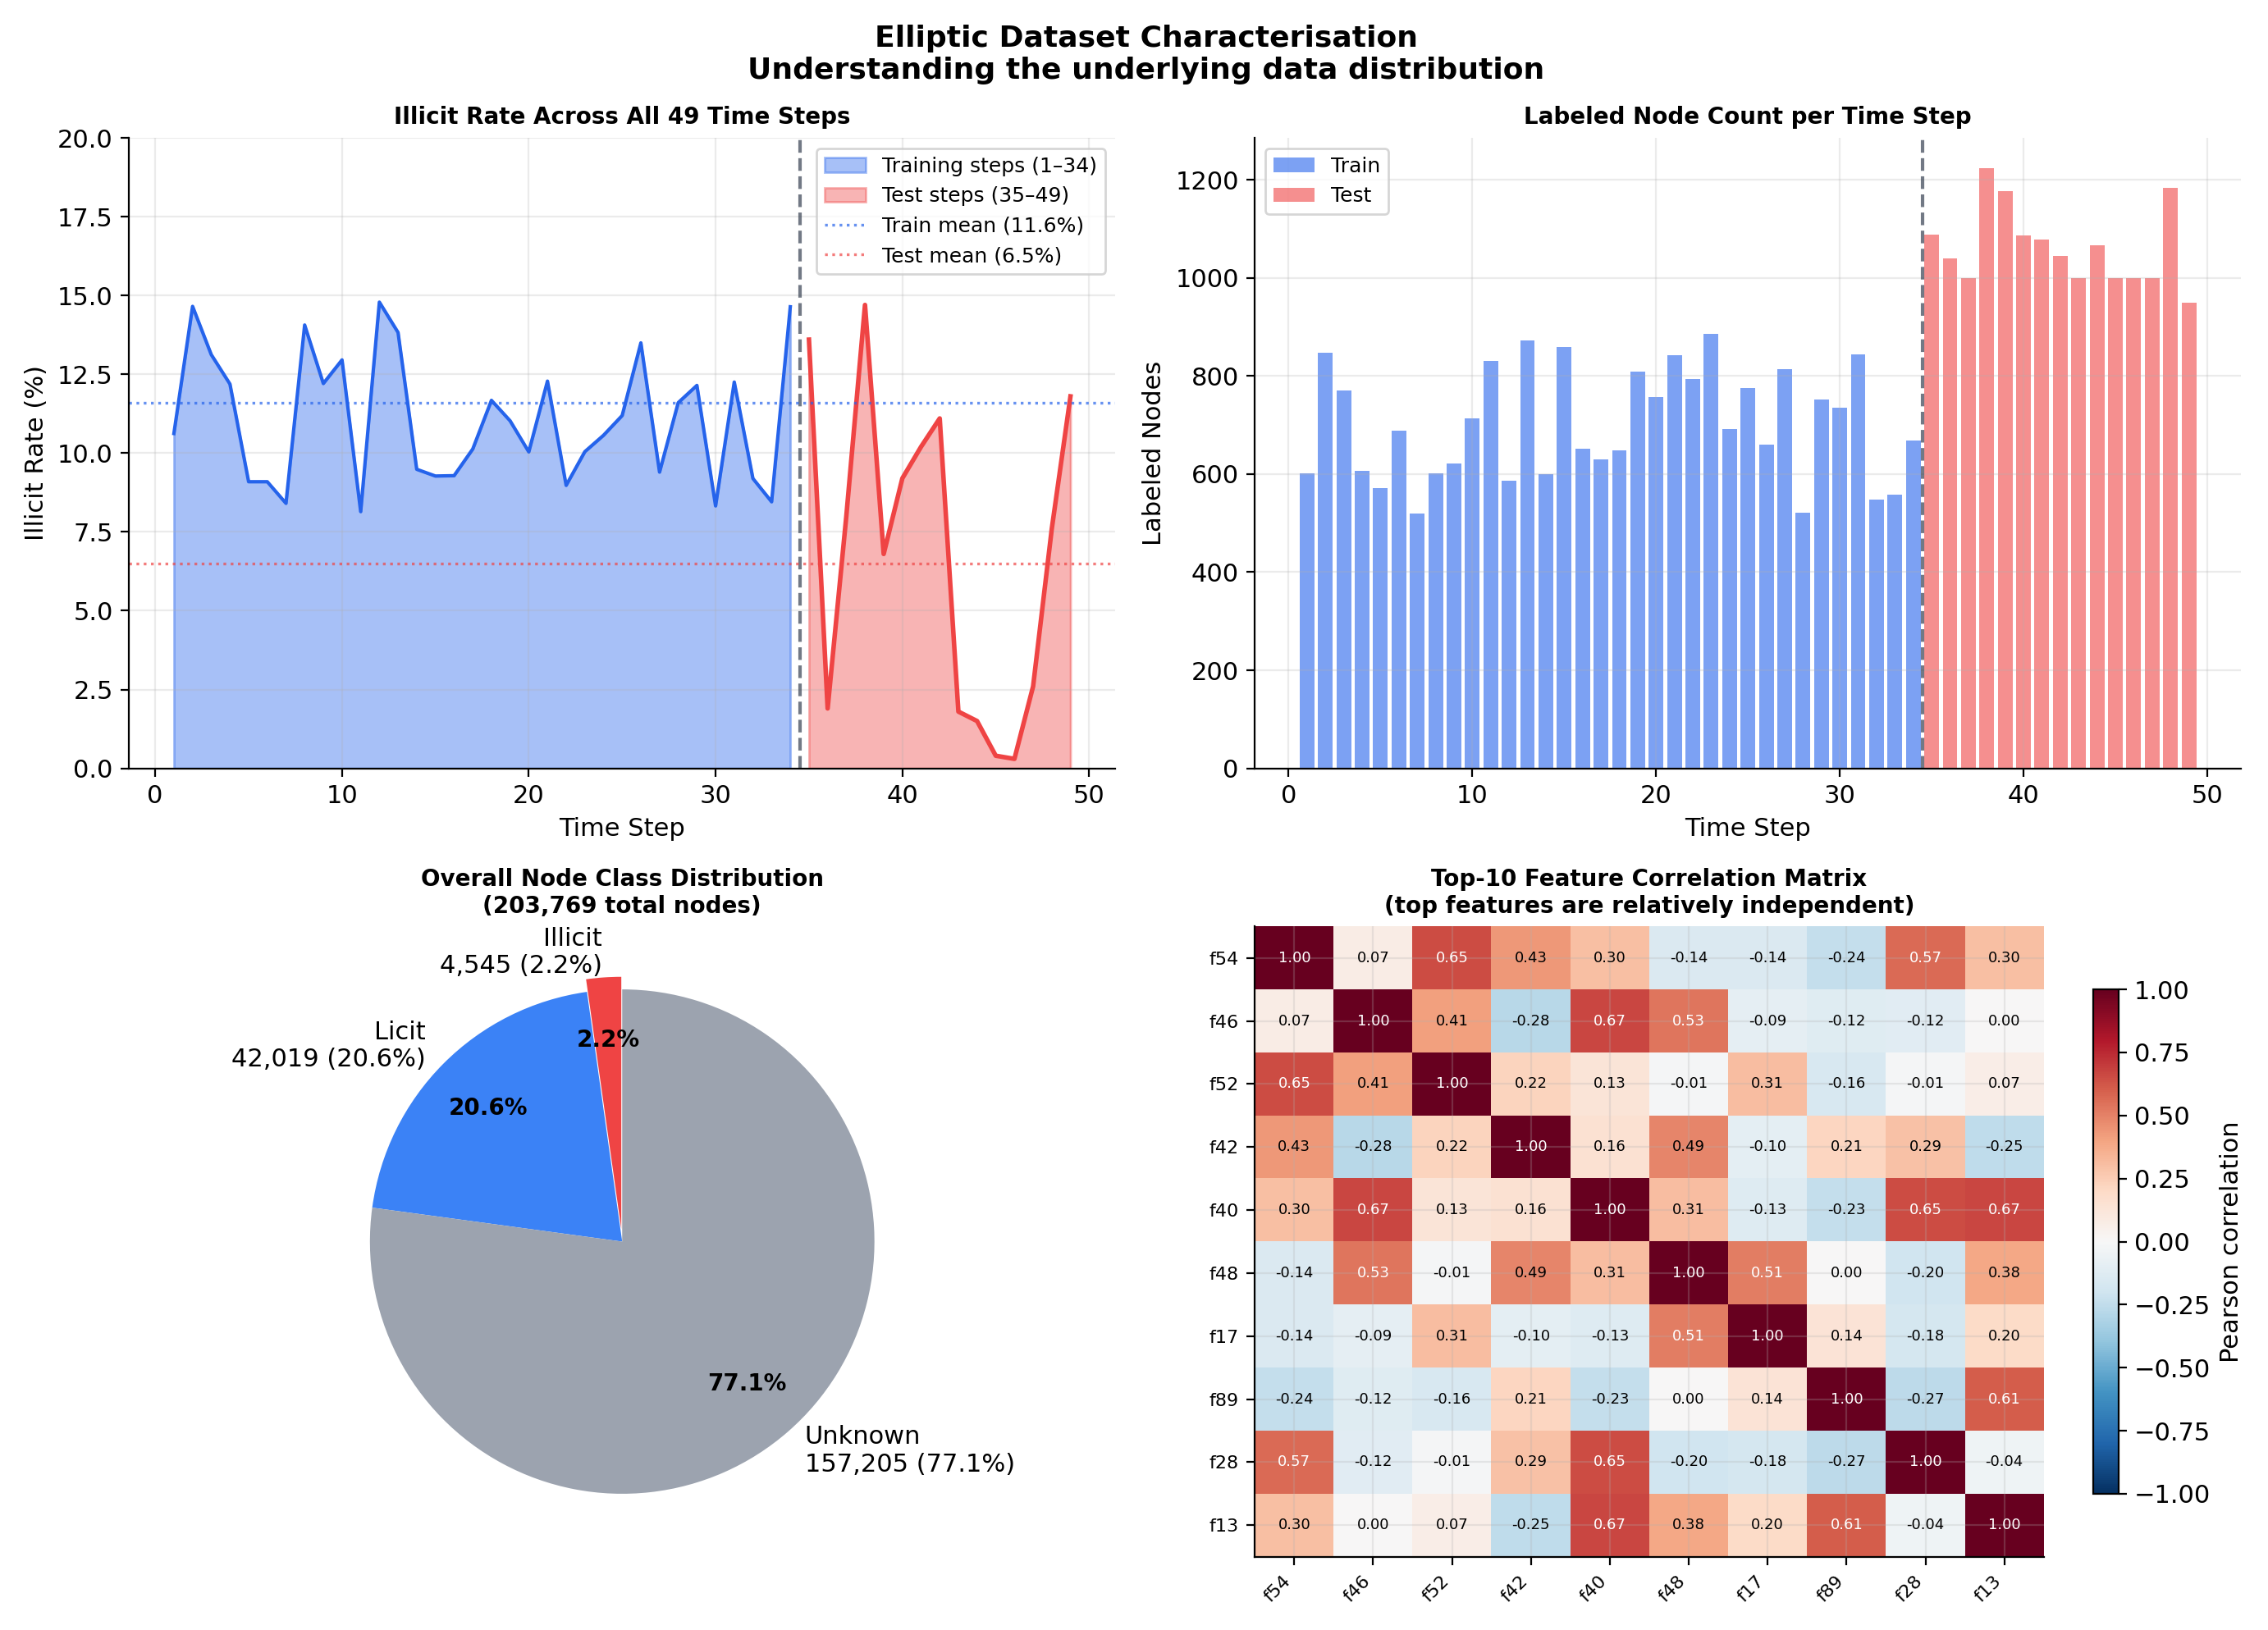
\includegraphics[width=\linewidth]{fig17_dataset_analysis.png}
\caption{Dataset characterisation. The temporal split coincides with a marked
change in illicit-rate behaviour, and the strongest features remain informative
without collapsing into a single redundant block.}
\label{fig:dataset_char}
\end{figure}

\subsection{Models, strategies, and evaluation}

We compare an MLP, GCN, GraphSAGE, GAT, and a CPU-constrained EvolveGCN
ablation. The MLP acts as the feature-only control. The GNNs use the same node
features plus learned neighbourhood aggregation. We evaluate three imbalance
strategies: Baseline cross-entropy, Weighted cross-entropy, and graph
augmentation. The main metric is illicit-class F1, reported as mean\,$\pm$\,std
across three seeds.

Evaluation is inductive. We use random-node mini-batches so that the model does
not access future test neighbourhoods during training. This is stricter than
the transductive setup used in prior Elliptic work.

\section{Results}

\subsection{Main benchmark}

Figure~\ref{fig:main_results} and Table~\ref{tab:main_results} summarise the
main comparison. The MLP is the best model in aggregate F1. GraphSAGE is the
strongest GNN, while GCN shows a large precision-recall imbalance.

\begin{figure}[!htbp]
\centering
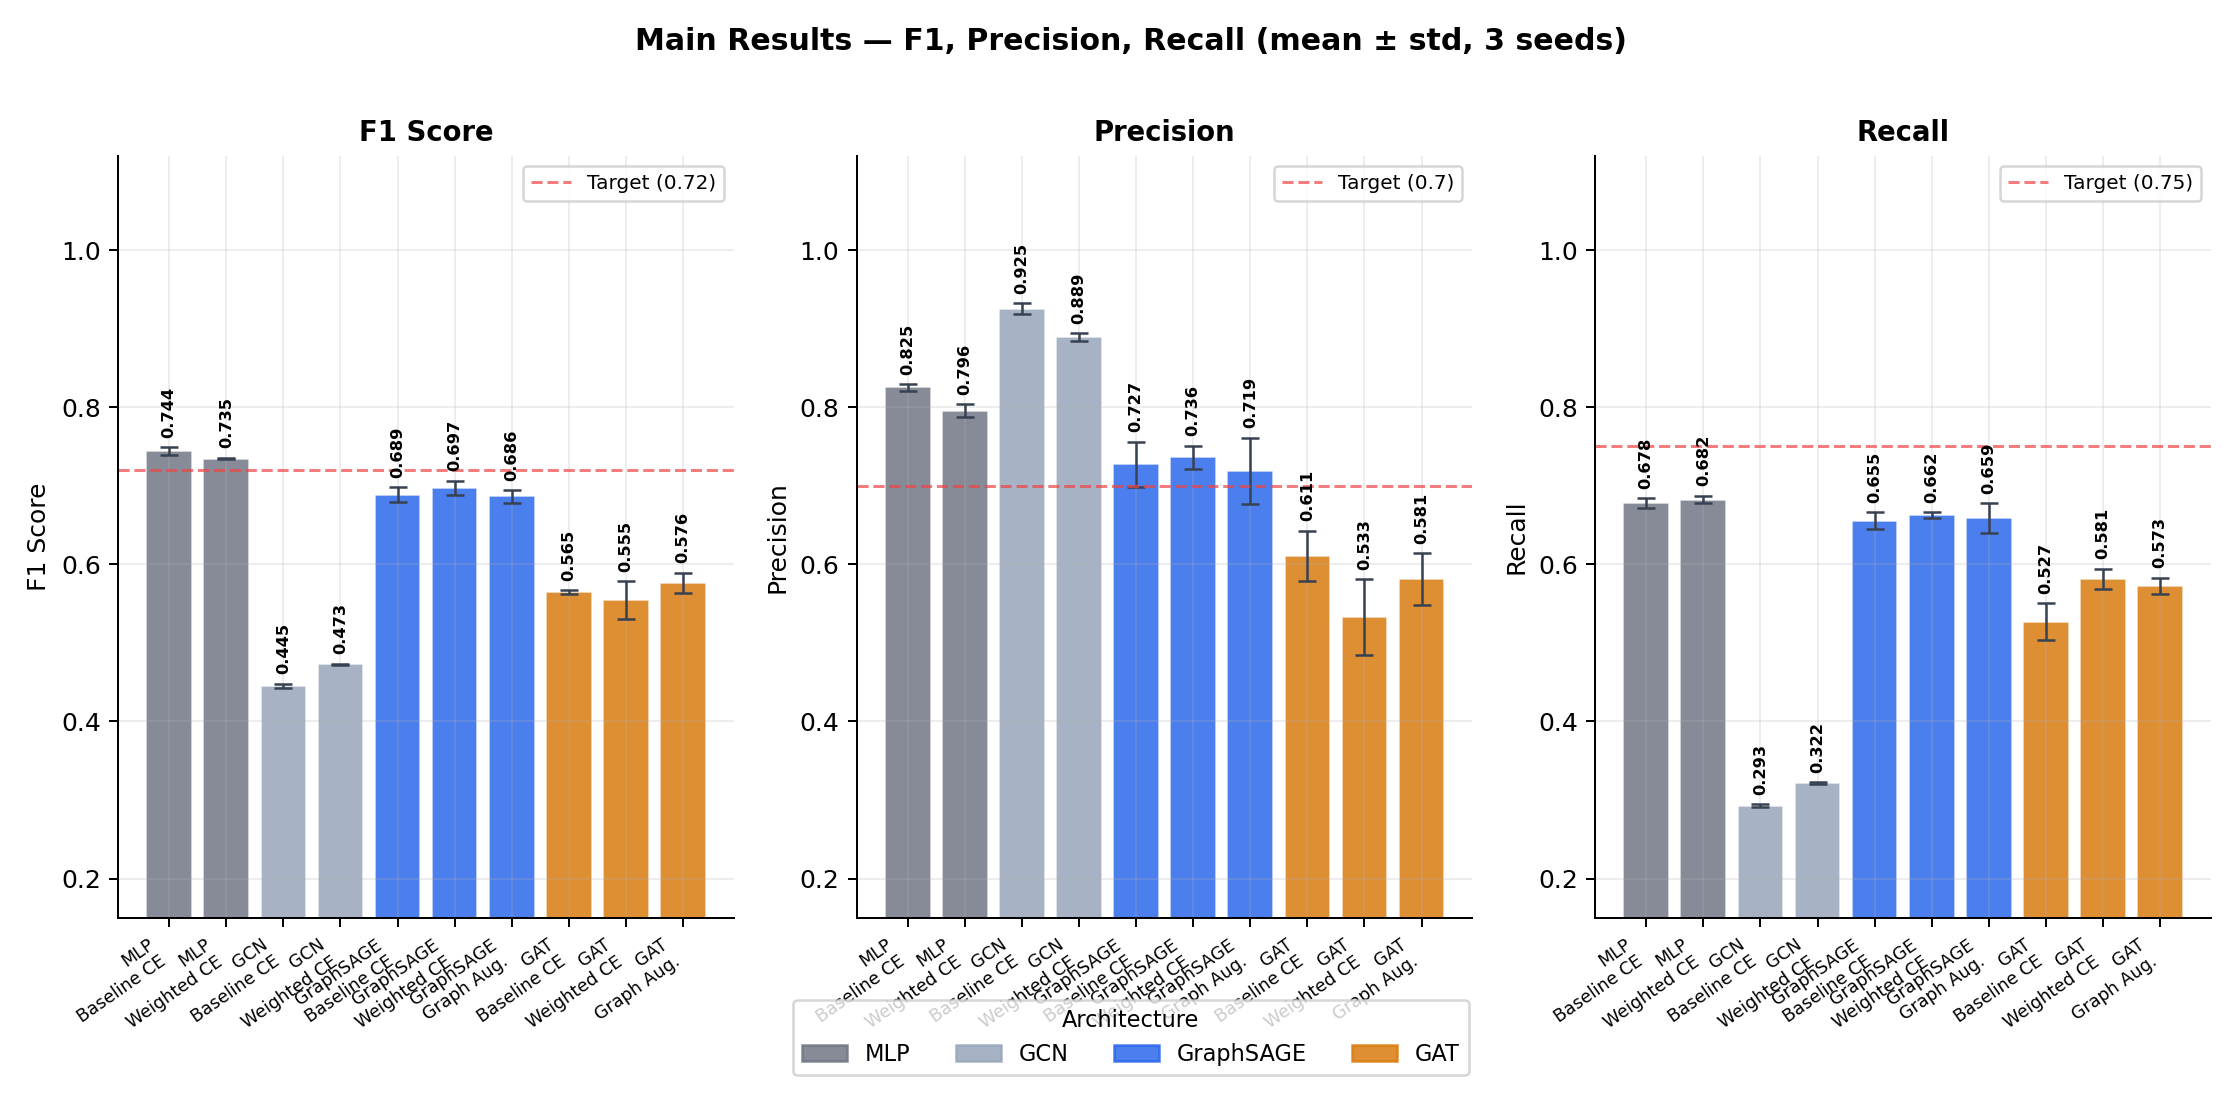
\includegraphics[width=\linewidth]{fig1_main_results.png}
\caption{Main benchmark across all configurations.}
\label{fig:main_results}
\end{figure}

\begin{table}[!htbp]
\centering
\caption{Main benchmark results (mean\,$\pm$\,std, 3 seeds).}
\label{tab:main_results}
\small
\resizebox{\linewidth}{!}{%
\begin{tabular}{llrrrr}
\toprule
\textbf{Model} & \textbf{Strategy} & \textbf{F1} & \textbf{Prec.} &
\textbf{Rec.} & \textbf{AUC} \\
\midrule
\multirow{2}{*}{MLP}
& Baseline & $\mathbf{0.744\pm0.005}$ & $\mathbf{0.825\pm0.004}$ &
$0.678\pm0.006$ & $0.891\pm0.001$ \\
& Weighted & $0.735\pm0.001$ & $0.796\pm0.008$ &
$0.682\pm0.005$ & $\mathbf{0.893\pm0.006}$ \\
\midrule
\multirow{2}{*}{GCN}
& Baseline & $0.445\pm0.003$ & $0.925\pm0.007$ &
$0.293\pm0.002$ & $0.868\pm0.009$ \\
& Weighted & $0.473\pm0.001$ & $0.889\pm0.005$ &
$0.322\pm0.001$ & $0.872\pm0.004$ \\
\midrule
\multirow{3}{*}{GraphSAGE}
& Baseline & $0.689\pm0.009$ & $0.727\pm0.029$ &
$0.655\pm0.011$ & $0.867\pm0.006$ \\
& Weighted & $0.697\pm0.009$ & $0.736\pm0.015$ &
$0.662\pm0.004$ & $0.868\pm0.003$ \\
& Graph Aug. & $0.686\pm0.008$ & $0.719\pm0.042$ &
$0.659\pm0.019$ & $0.861\pm0.007$ \\
\midrule
\multirow{3}{*}{GAT}
& Baseline & $0.565\pm0.002$ & $0.611\pm0.032$ &
$0.527\pm0.023$ & $0.863\pm0.007$ \\
& Weighted & $0.555\pm0.024$ & $0.533\pm0.048$ &
$\mathbf{0.581\pm0.013}$ & $0.855\pm0.004$ \\
& Graph Aug. & $0.576\pm0.013$ & $0.581\pm0.033$ &
$0.573\pm0.010$ & $0.842\pm0.002$ \\
\bottomrule
\end{tabular}
}
\end{table}

\subsection{Strategy sensitivity and robustness}

Figure~\ref{fig:strategy_variance} reorganises the benchmark around the
imbalance strategy and the seed variance. The main point is that architecture
matters more than strategy in the final ranking, although the strategy changes
the precision-recall trade-off.

\begin{figure}[!htbp]
\centering
\begin{minipage}[b]{0.48\linewidth}
  \centering
  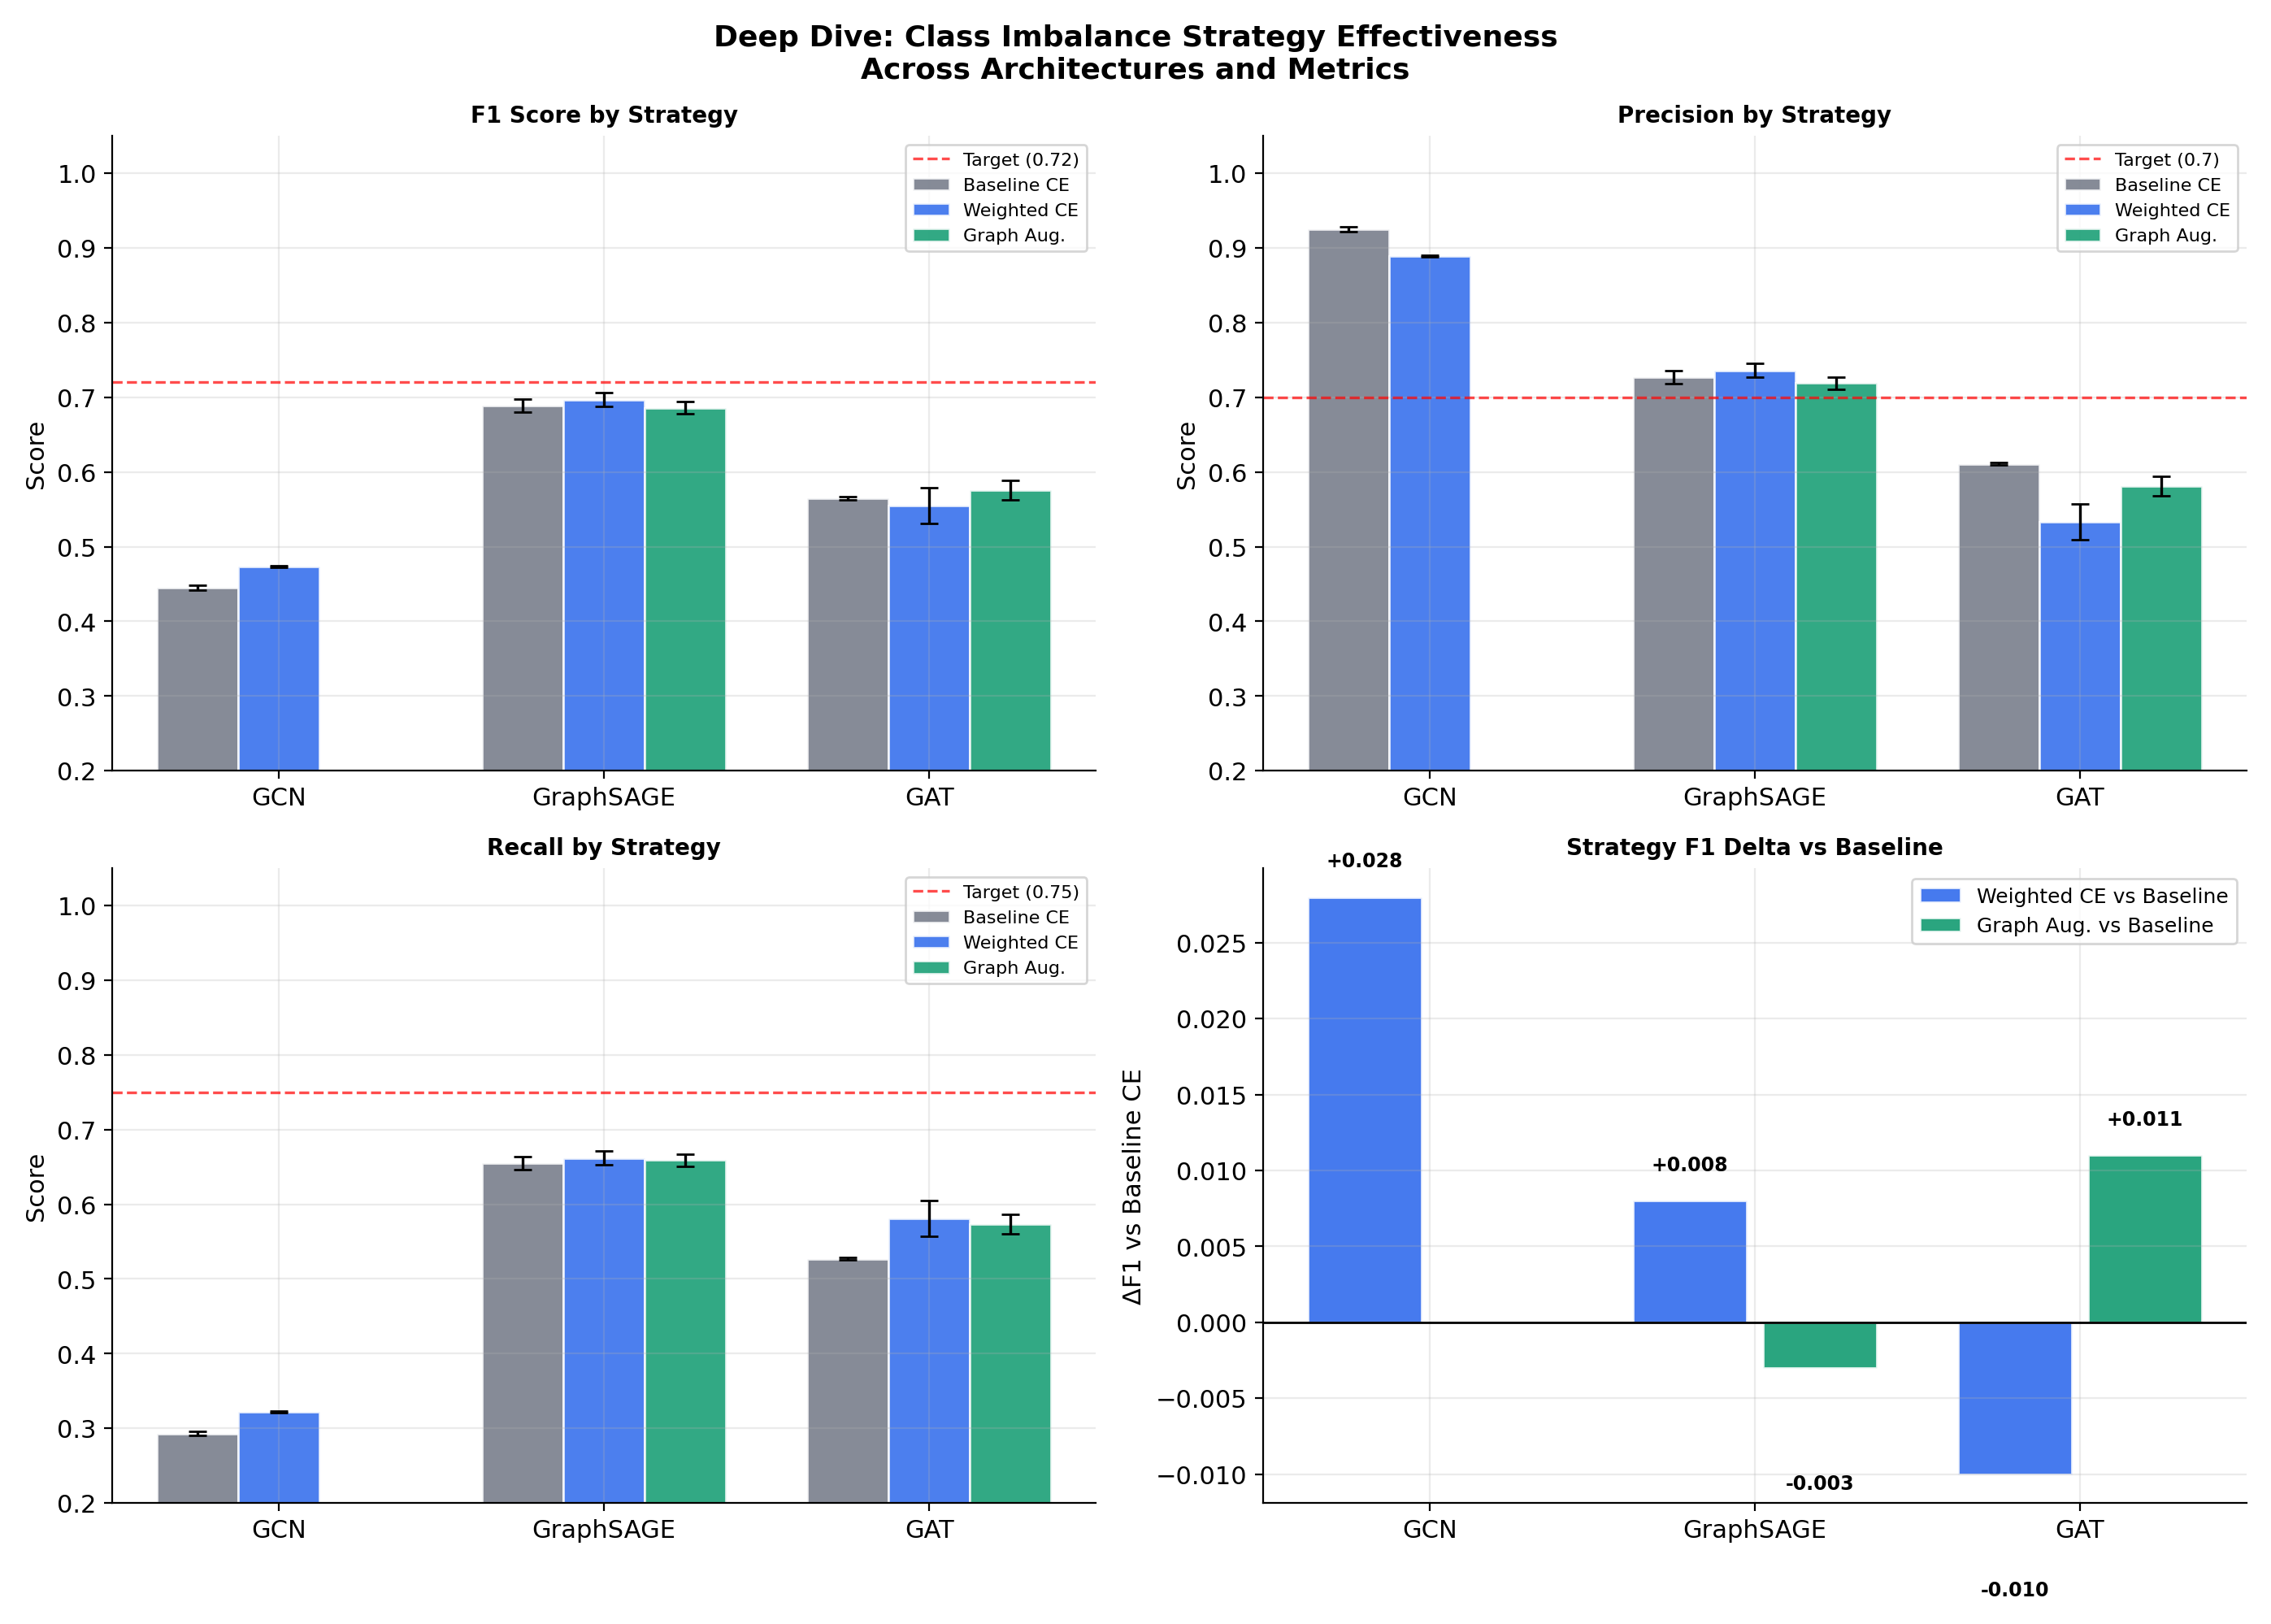
\includegraphics[width=\linewidth]{fig14_strategy_deep_dive.png}\\[-0.2em]
  \footnotesize\textbf{(a)} Strategy deep-dive.
\end{minipage}
\hfill
\begin{minipage}[b]{0.48\linewidth}
  \centering
  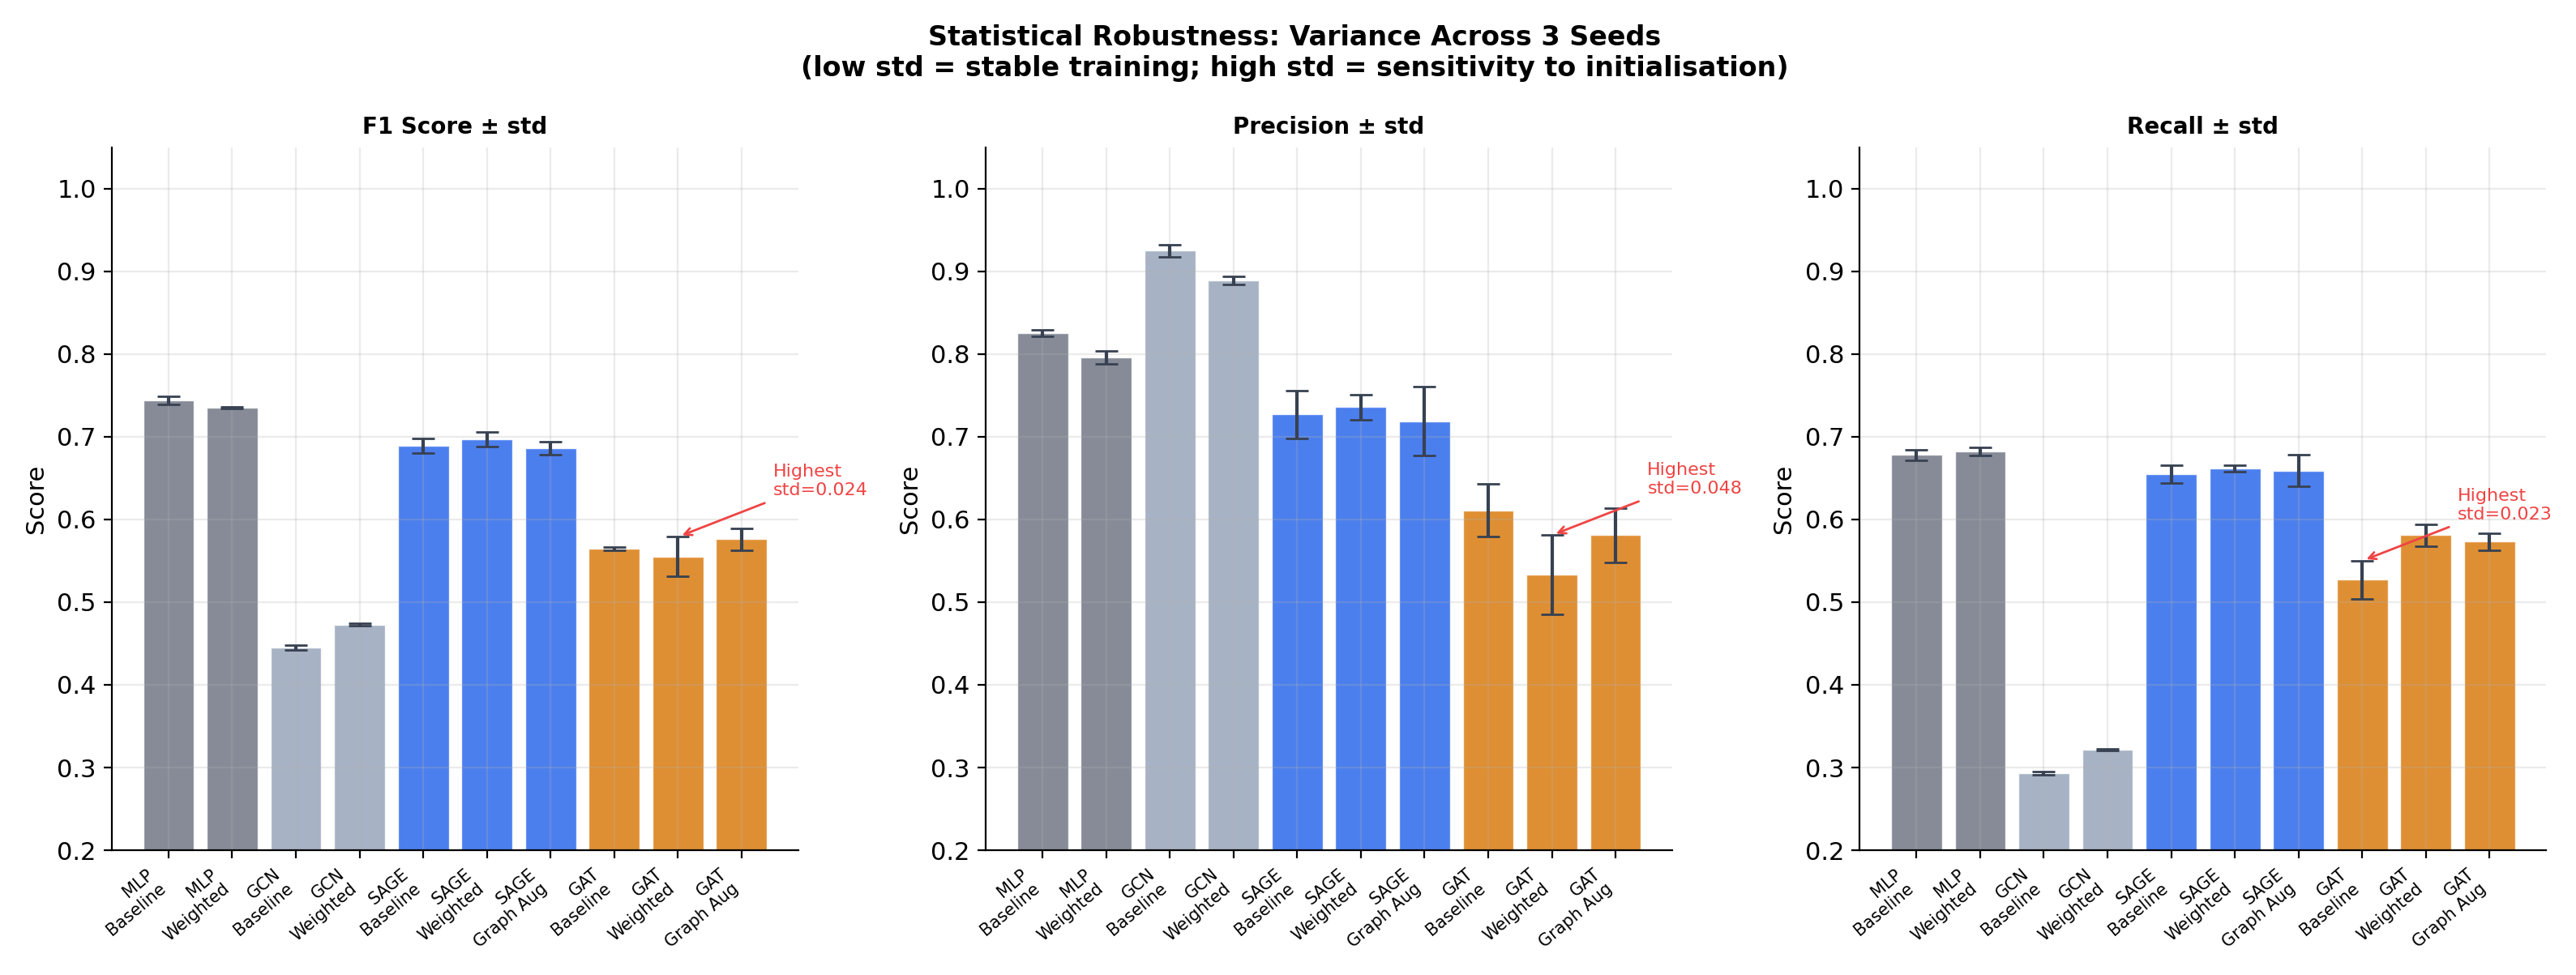
\includegraphics[width=\linewidth]{fig15_variance_analysis.png}\\[-0.2em]
  \footnotesize\textbf{(b)} Variance across seeds.
\end{minipage}
\caption{Strategy sensitivity and statistical robustness.}
\label{fig:strategy_variance}
\end{figure}

\subsection{Temporal collapse}

The central empirical result is temporal collapse. Figure~\ref{fig:temporal}
shows that every model degrades sharply after step~42, which is exactly where
the test period moves into a lower-fraud regime.

\begin{figure}[!htbp]
\centering
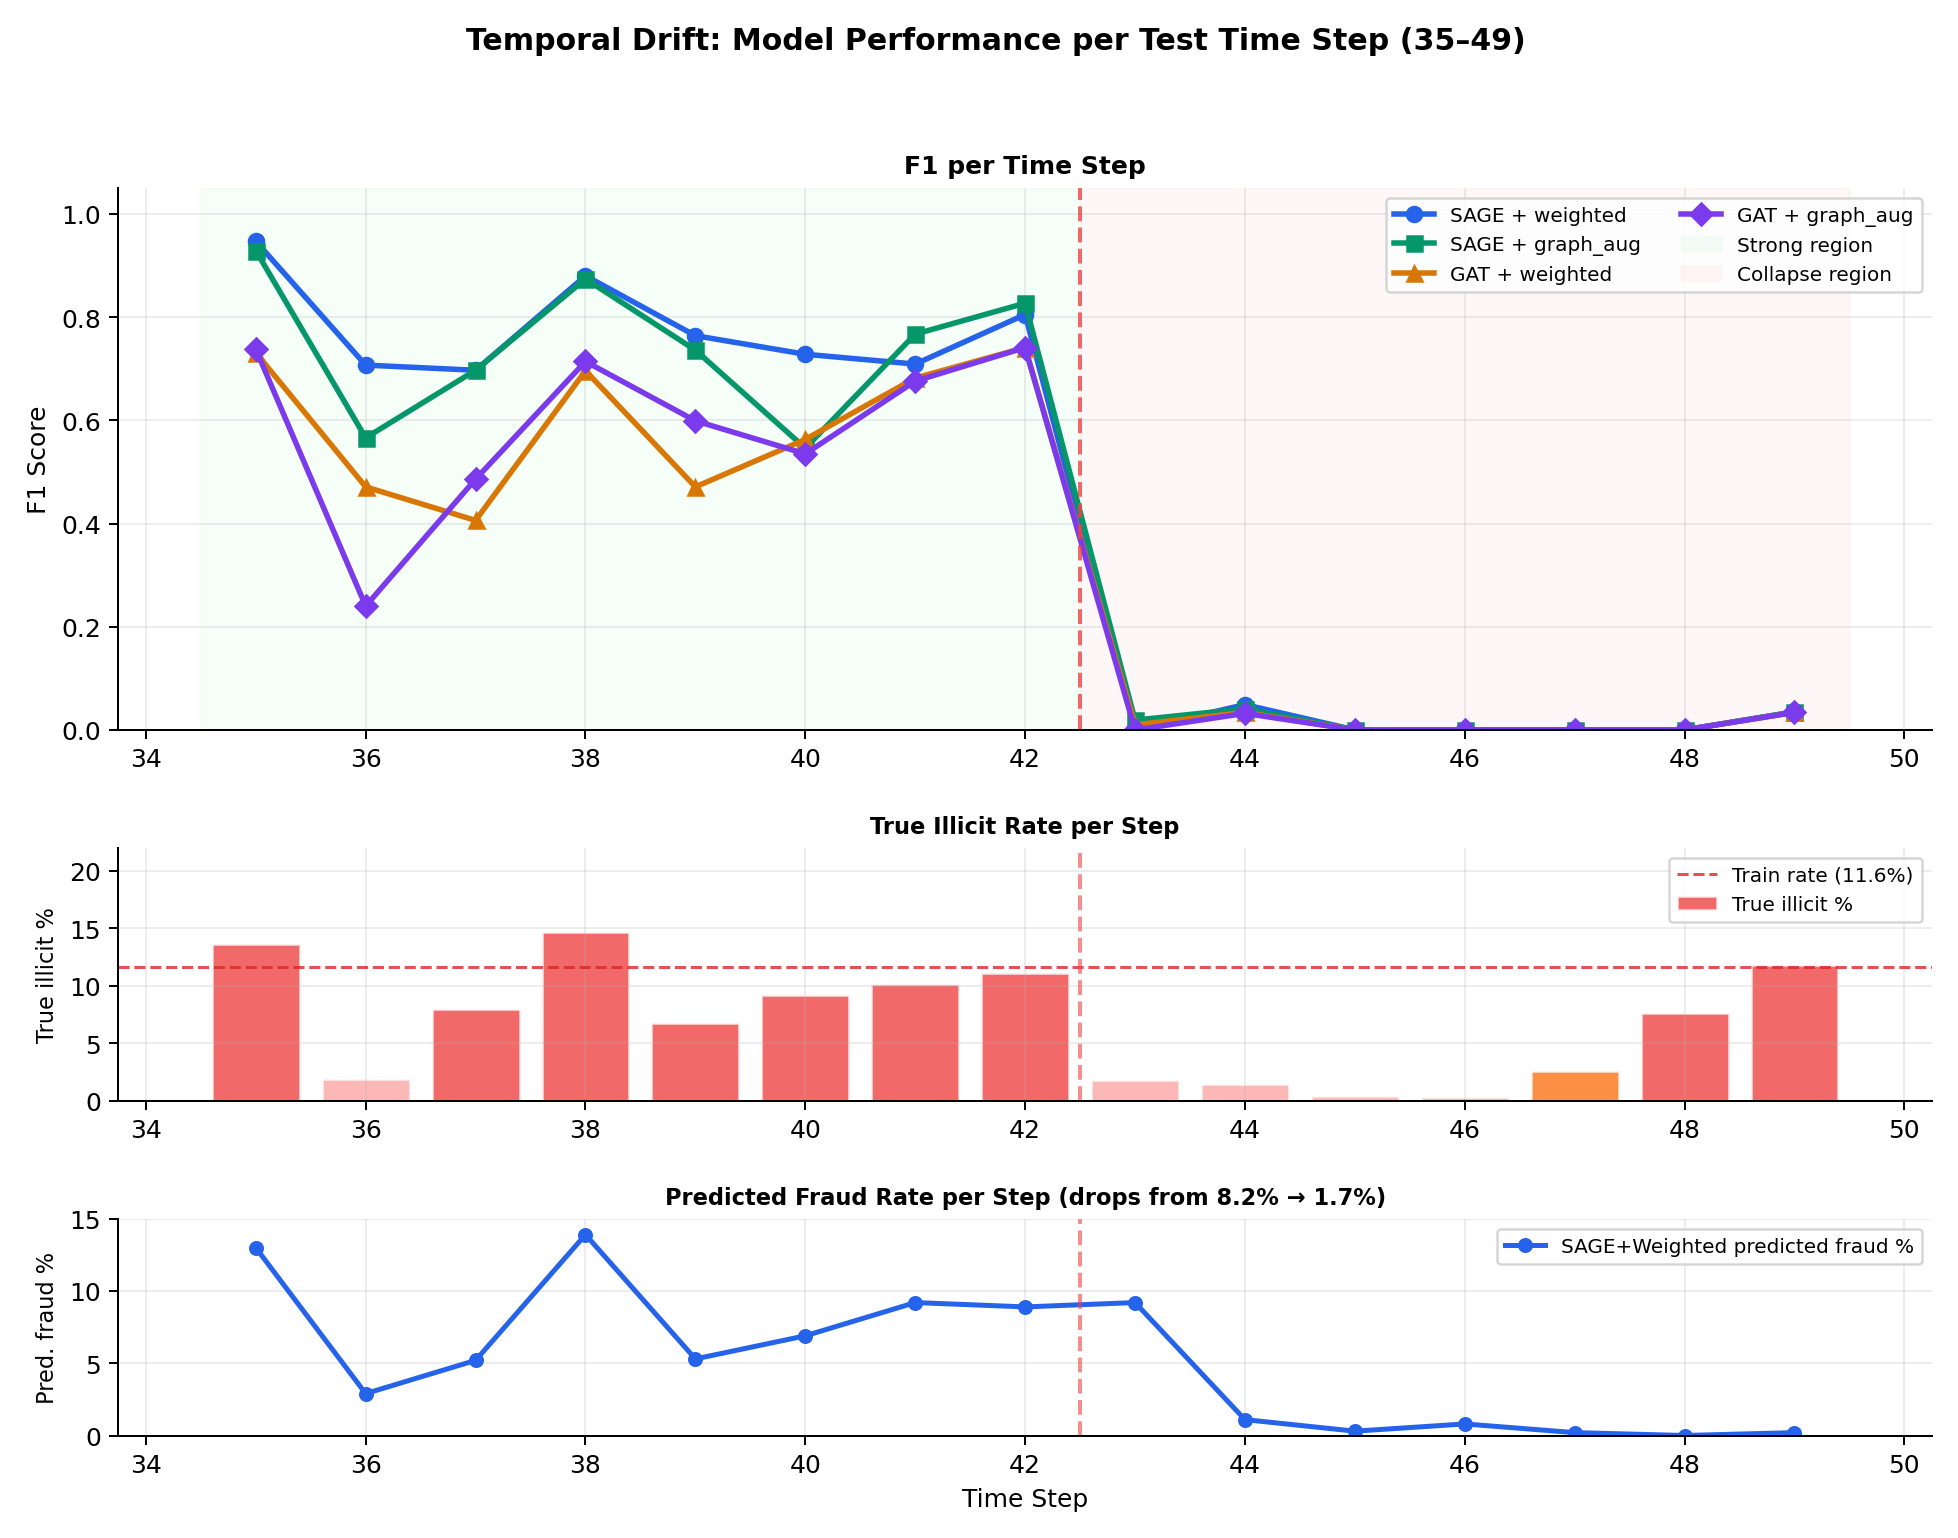
\includegraphics[width=\linewidth]{fig2_temporal_drift.png}
\caption{Per-step F1 and illicit-rate shift across the test window.}
\label{fig:temporal}
\end{figure}

This is a recall failure rather than a generic loss of discrimination. The
models become increasingly conservative and stop predicting fraud in the late
steps. Temperature scaling does not repair the collapse.

\subsection{Why the MLP stays ahead}

Figure~\ref{fig:features_community} shows two parts of the explanation. Local
transaction features dominate the Random Forest importance ranking, accounting
for 82.4\,\% of total importance, while fraud community structure is clearly
present in the graph. Figure~\ref{fig:ablation_advantage} connects those two
observations: graph structure can help briefly, but the advantage flips after
the regime change.

\begin{figure}[!htbp]
\centering
\begin{minipage}[b]{0.48\linewidth}
  \centering
  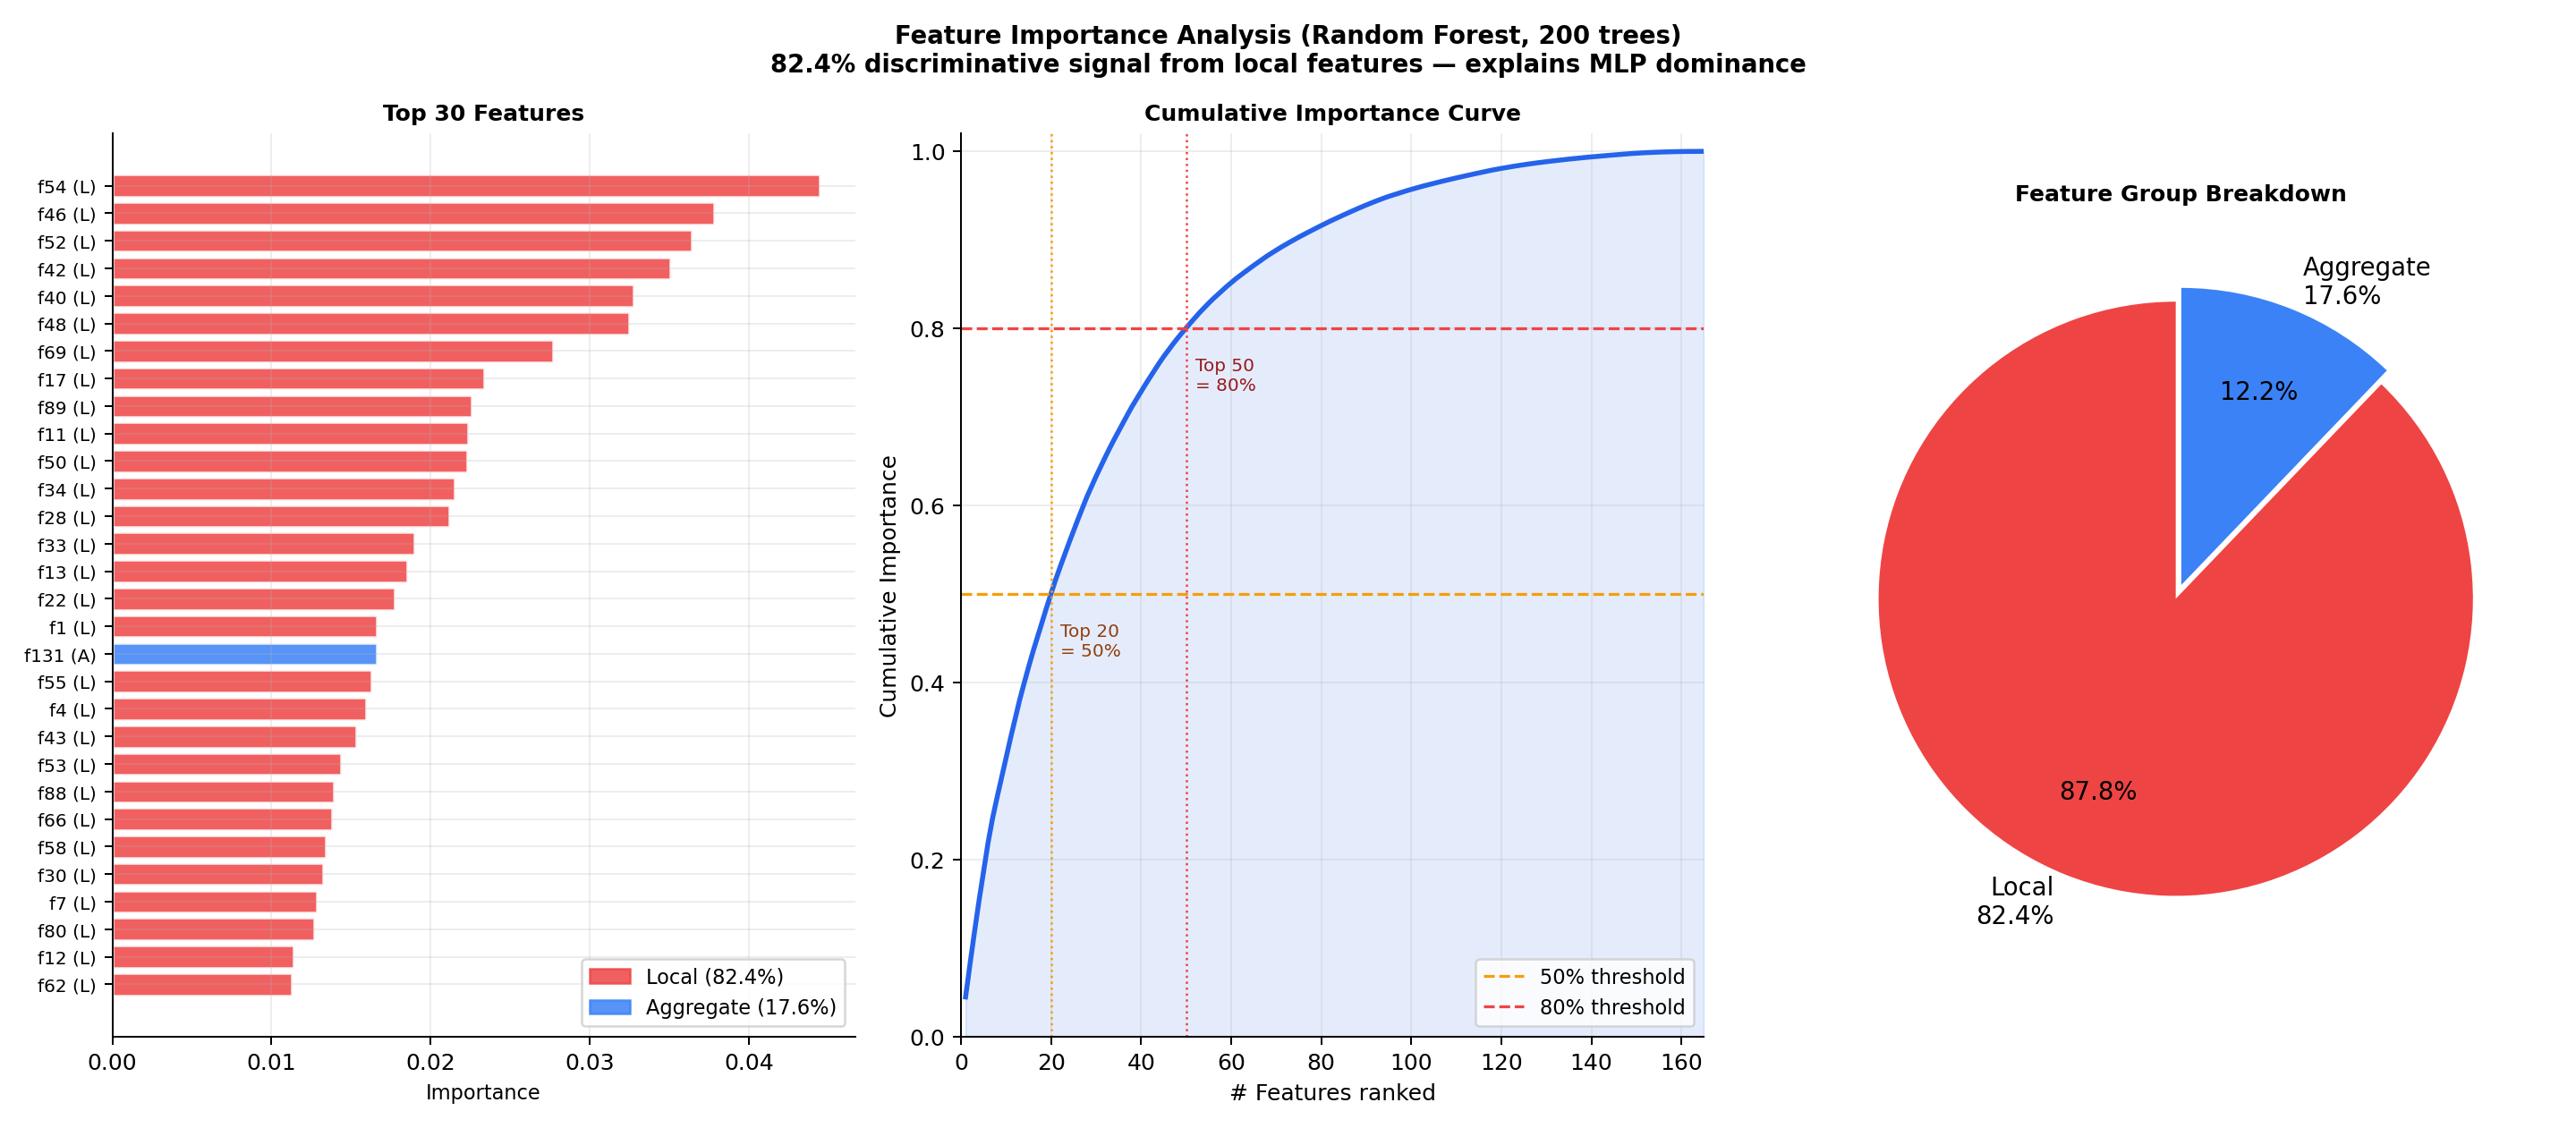
\includegraphics[width=\linewidth]{fig4_feature_importance.png}\\[-0.2em]
  \footnotesize\textbf{(a)} Feature attribution.
\end{minipage}
\hfill
\begin{minipage}[b]{0.48\linewidth}
  \centering
  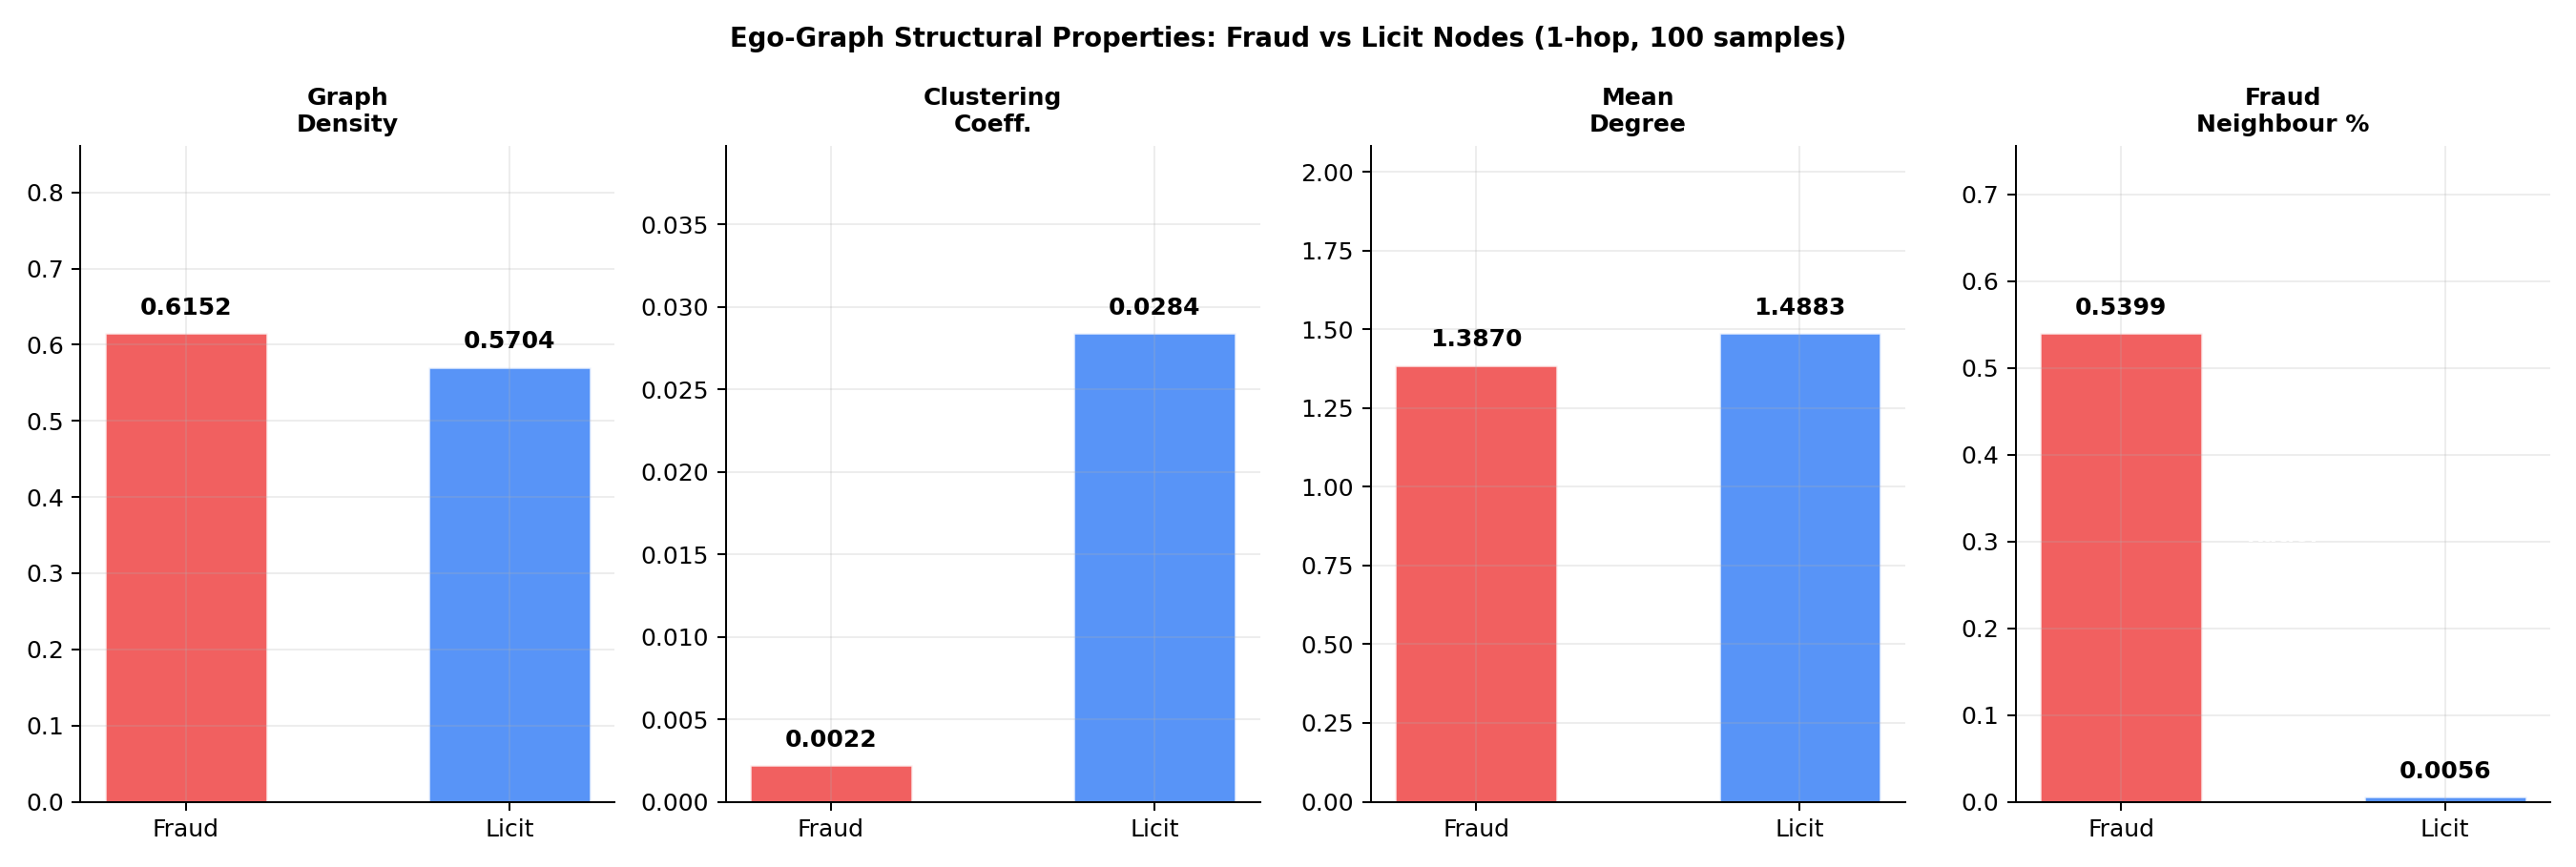
\includegraphics[width=\linewidth]{fig5_community_structure.png}\\[-0.2em]
  \footnotesize\textbf{(b)} Community structure.
\end{minipage}
\caption{Local features dominate the stable signal, while community structure
remains informative but temporally fragile.}
\label{fig:features_community}
\end{figure}

\begin{figure}[!htbp]
\centering
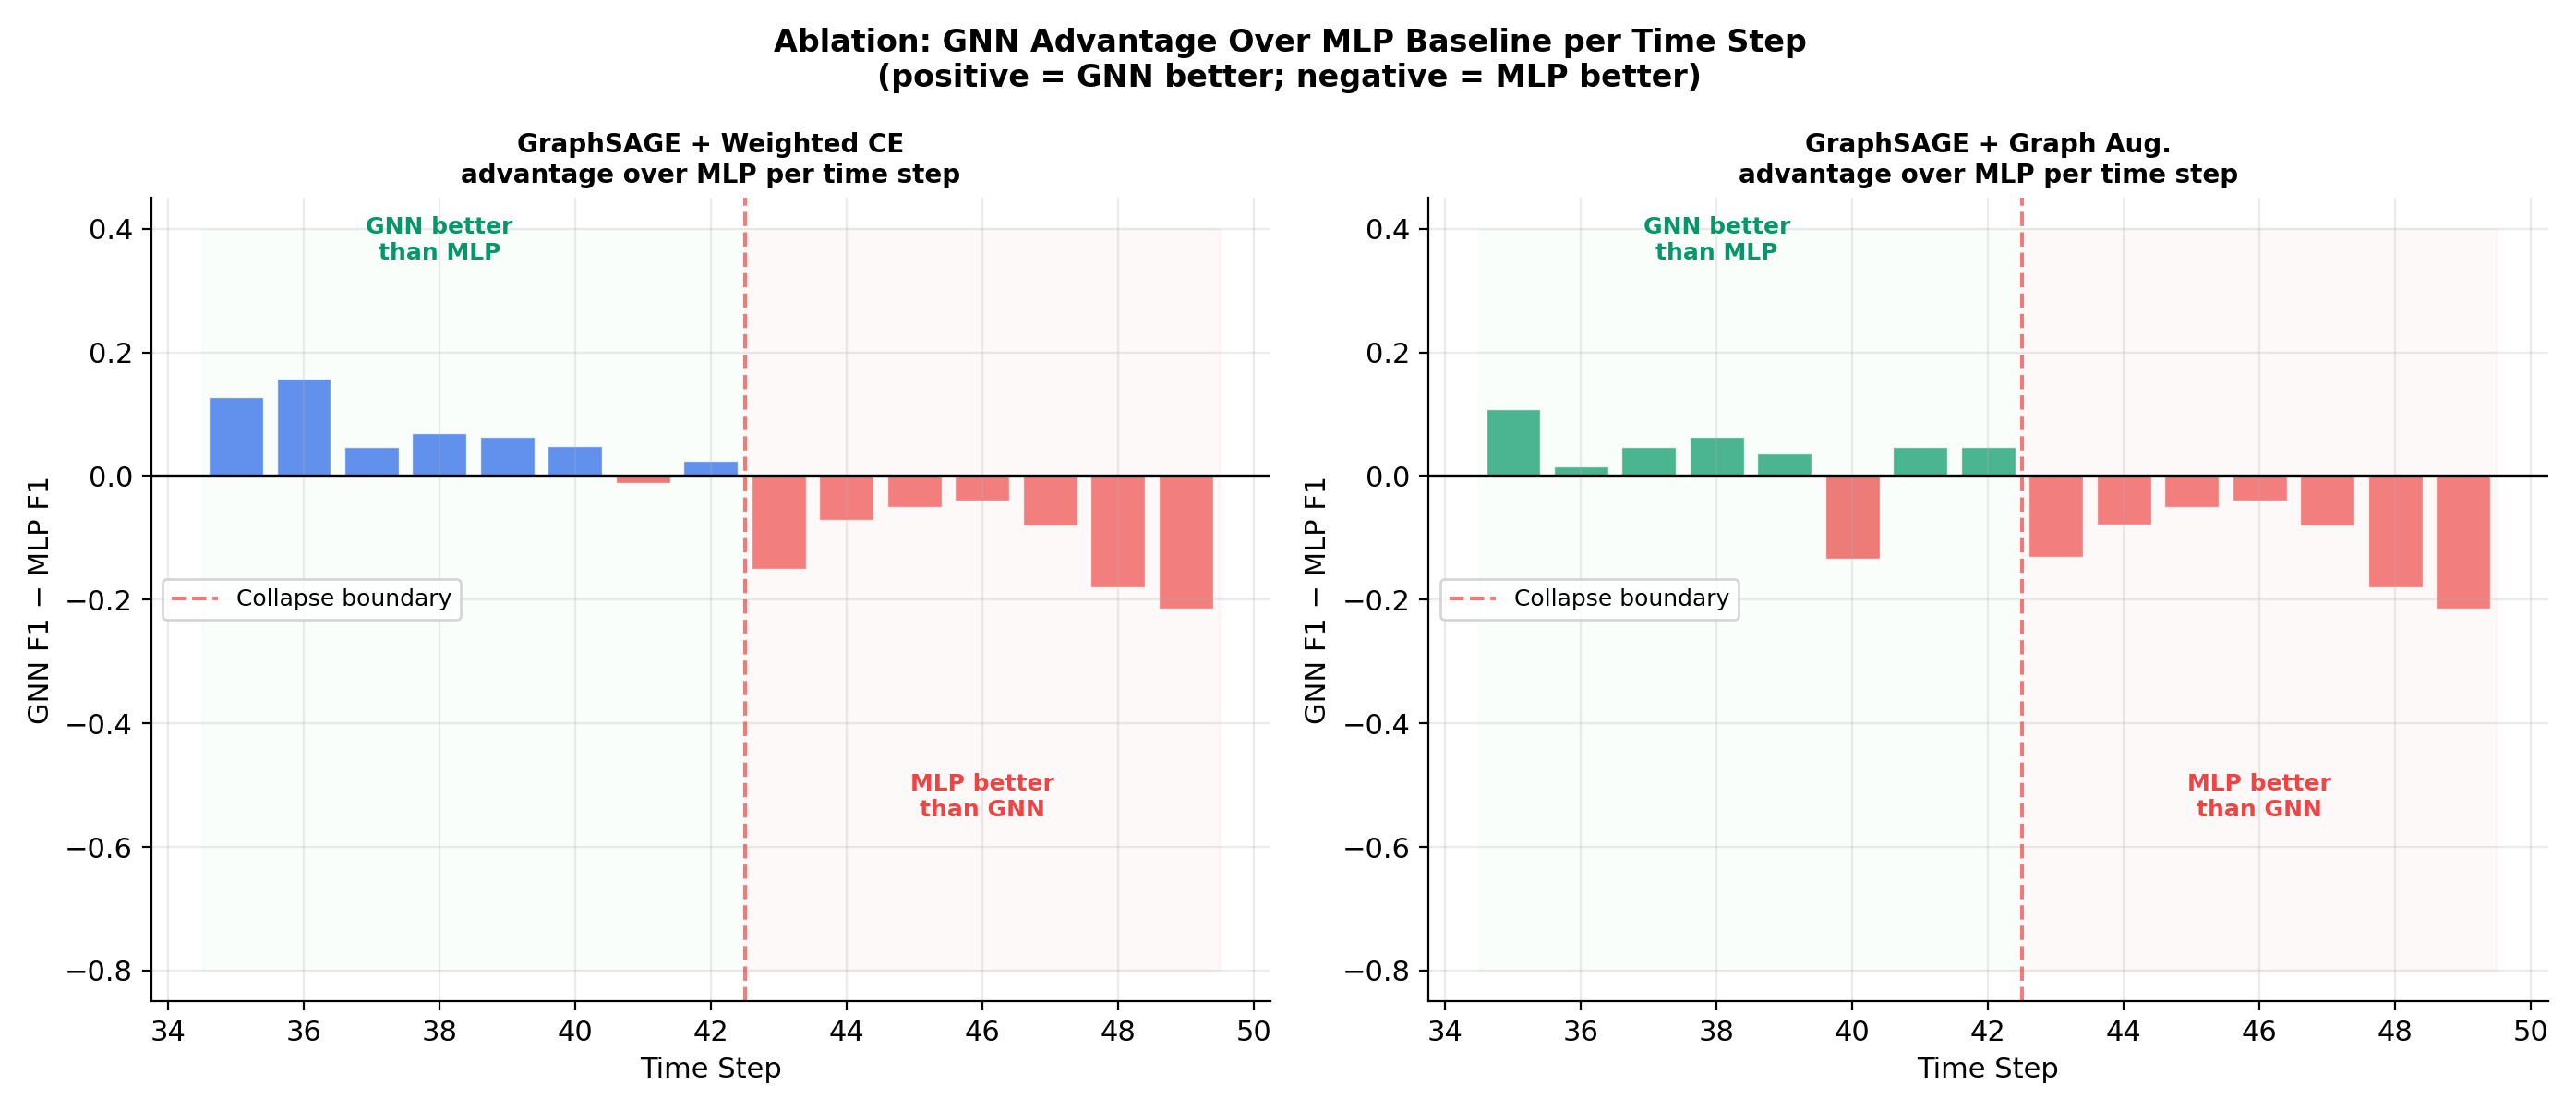
\includegraphics[width=\linewidth]{fig16_ablation_advantage.png}
\caption{Per-step GraphSAGE advantage over the MLP baseline. The sign reversal
after step~42 shows when graph structure turns from a short-term asset into a
liability.}
\label{fig:ablation_advantage}
\end{figure}

\section{Additional analyses}

Temperature scaling produces fitted temperatures in the mild-overconfidence
range, but it leaves F1 unchanged, which indicates that the failure is not a
simple calibration issue. The EvolveGCN ablation reaches F1\,=\,0.29 on CPU,
far below the published GPU result of 0.77, which shows how strongly temporal
architectures depend on full snapshots and adequate hardware. Business-cost
analysis under asymmetric penalties further shows that the highest-F1 model is
not always the most cost-effective one to deploy.

\begin{figure}[!htbp]
\centering
\begin{minipage}[b]{0.48\linewidth}
  \centering
  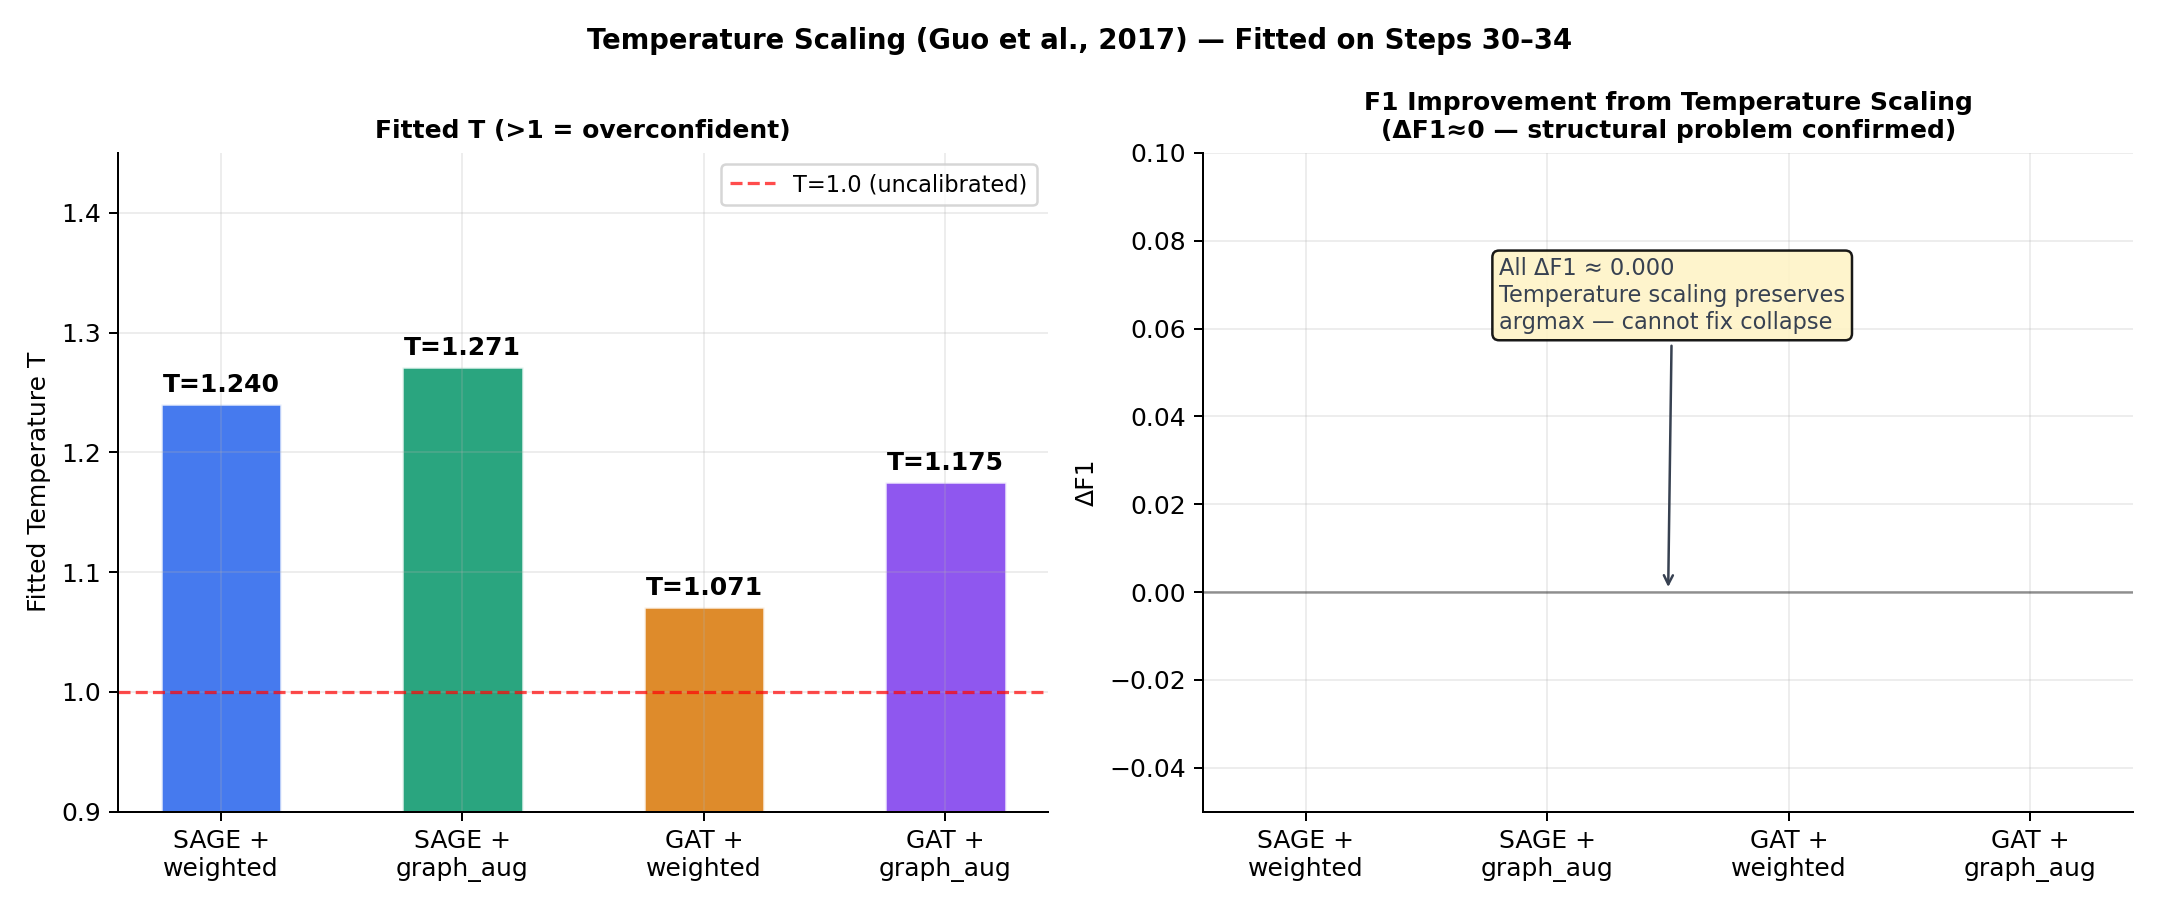
\includegraphics[width=\linewidth]{fig13_temperature_scaling.png}\\[-0.2em]
  \footnotesize\textbf{(a)} Temperature scaling.
\end{minipage}
\hfill
\begin{minipage}[b]{0.48\linewidth}
  \centering
  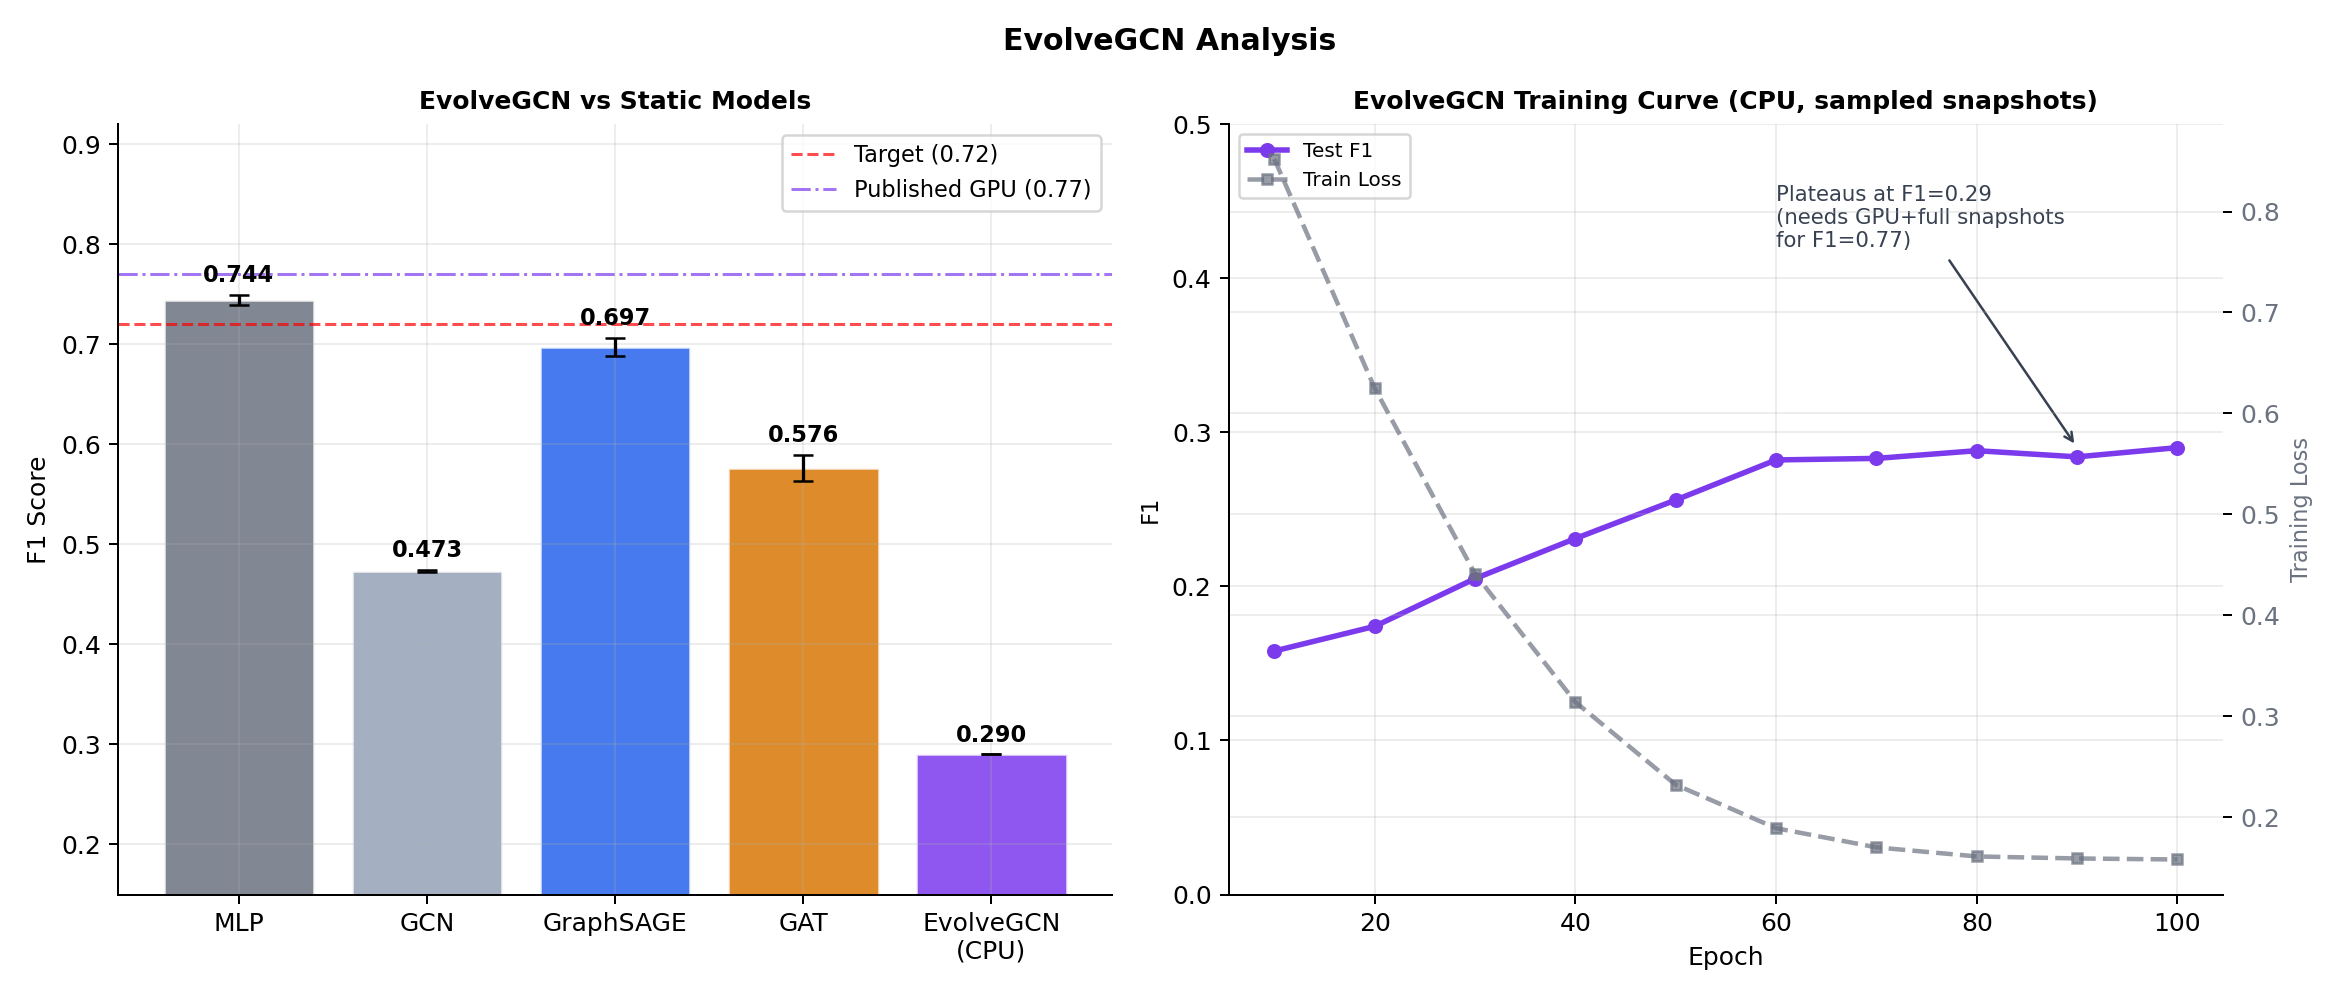
\includegraphics[width=\linewidth]{fig9_evolvegcn.png}\\[-0.2em]
  \footnotesize\textbf{(b)} EvolveGCN hardware ablation.
\end{minipage}
\caption{Post-hoc calibration does not recover performance, while temporal GNN
deployment remains hardware-sensitive.}
\label{fig:calibration_evolve}
\end{figure}

\begin{figure}[!t]
\centering
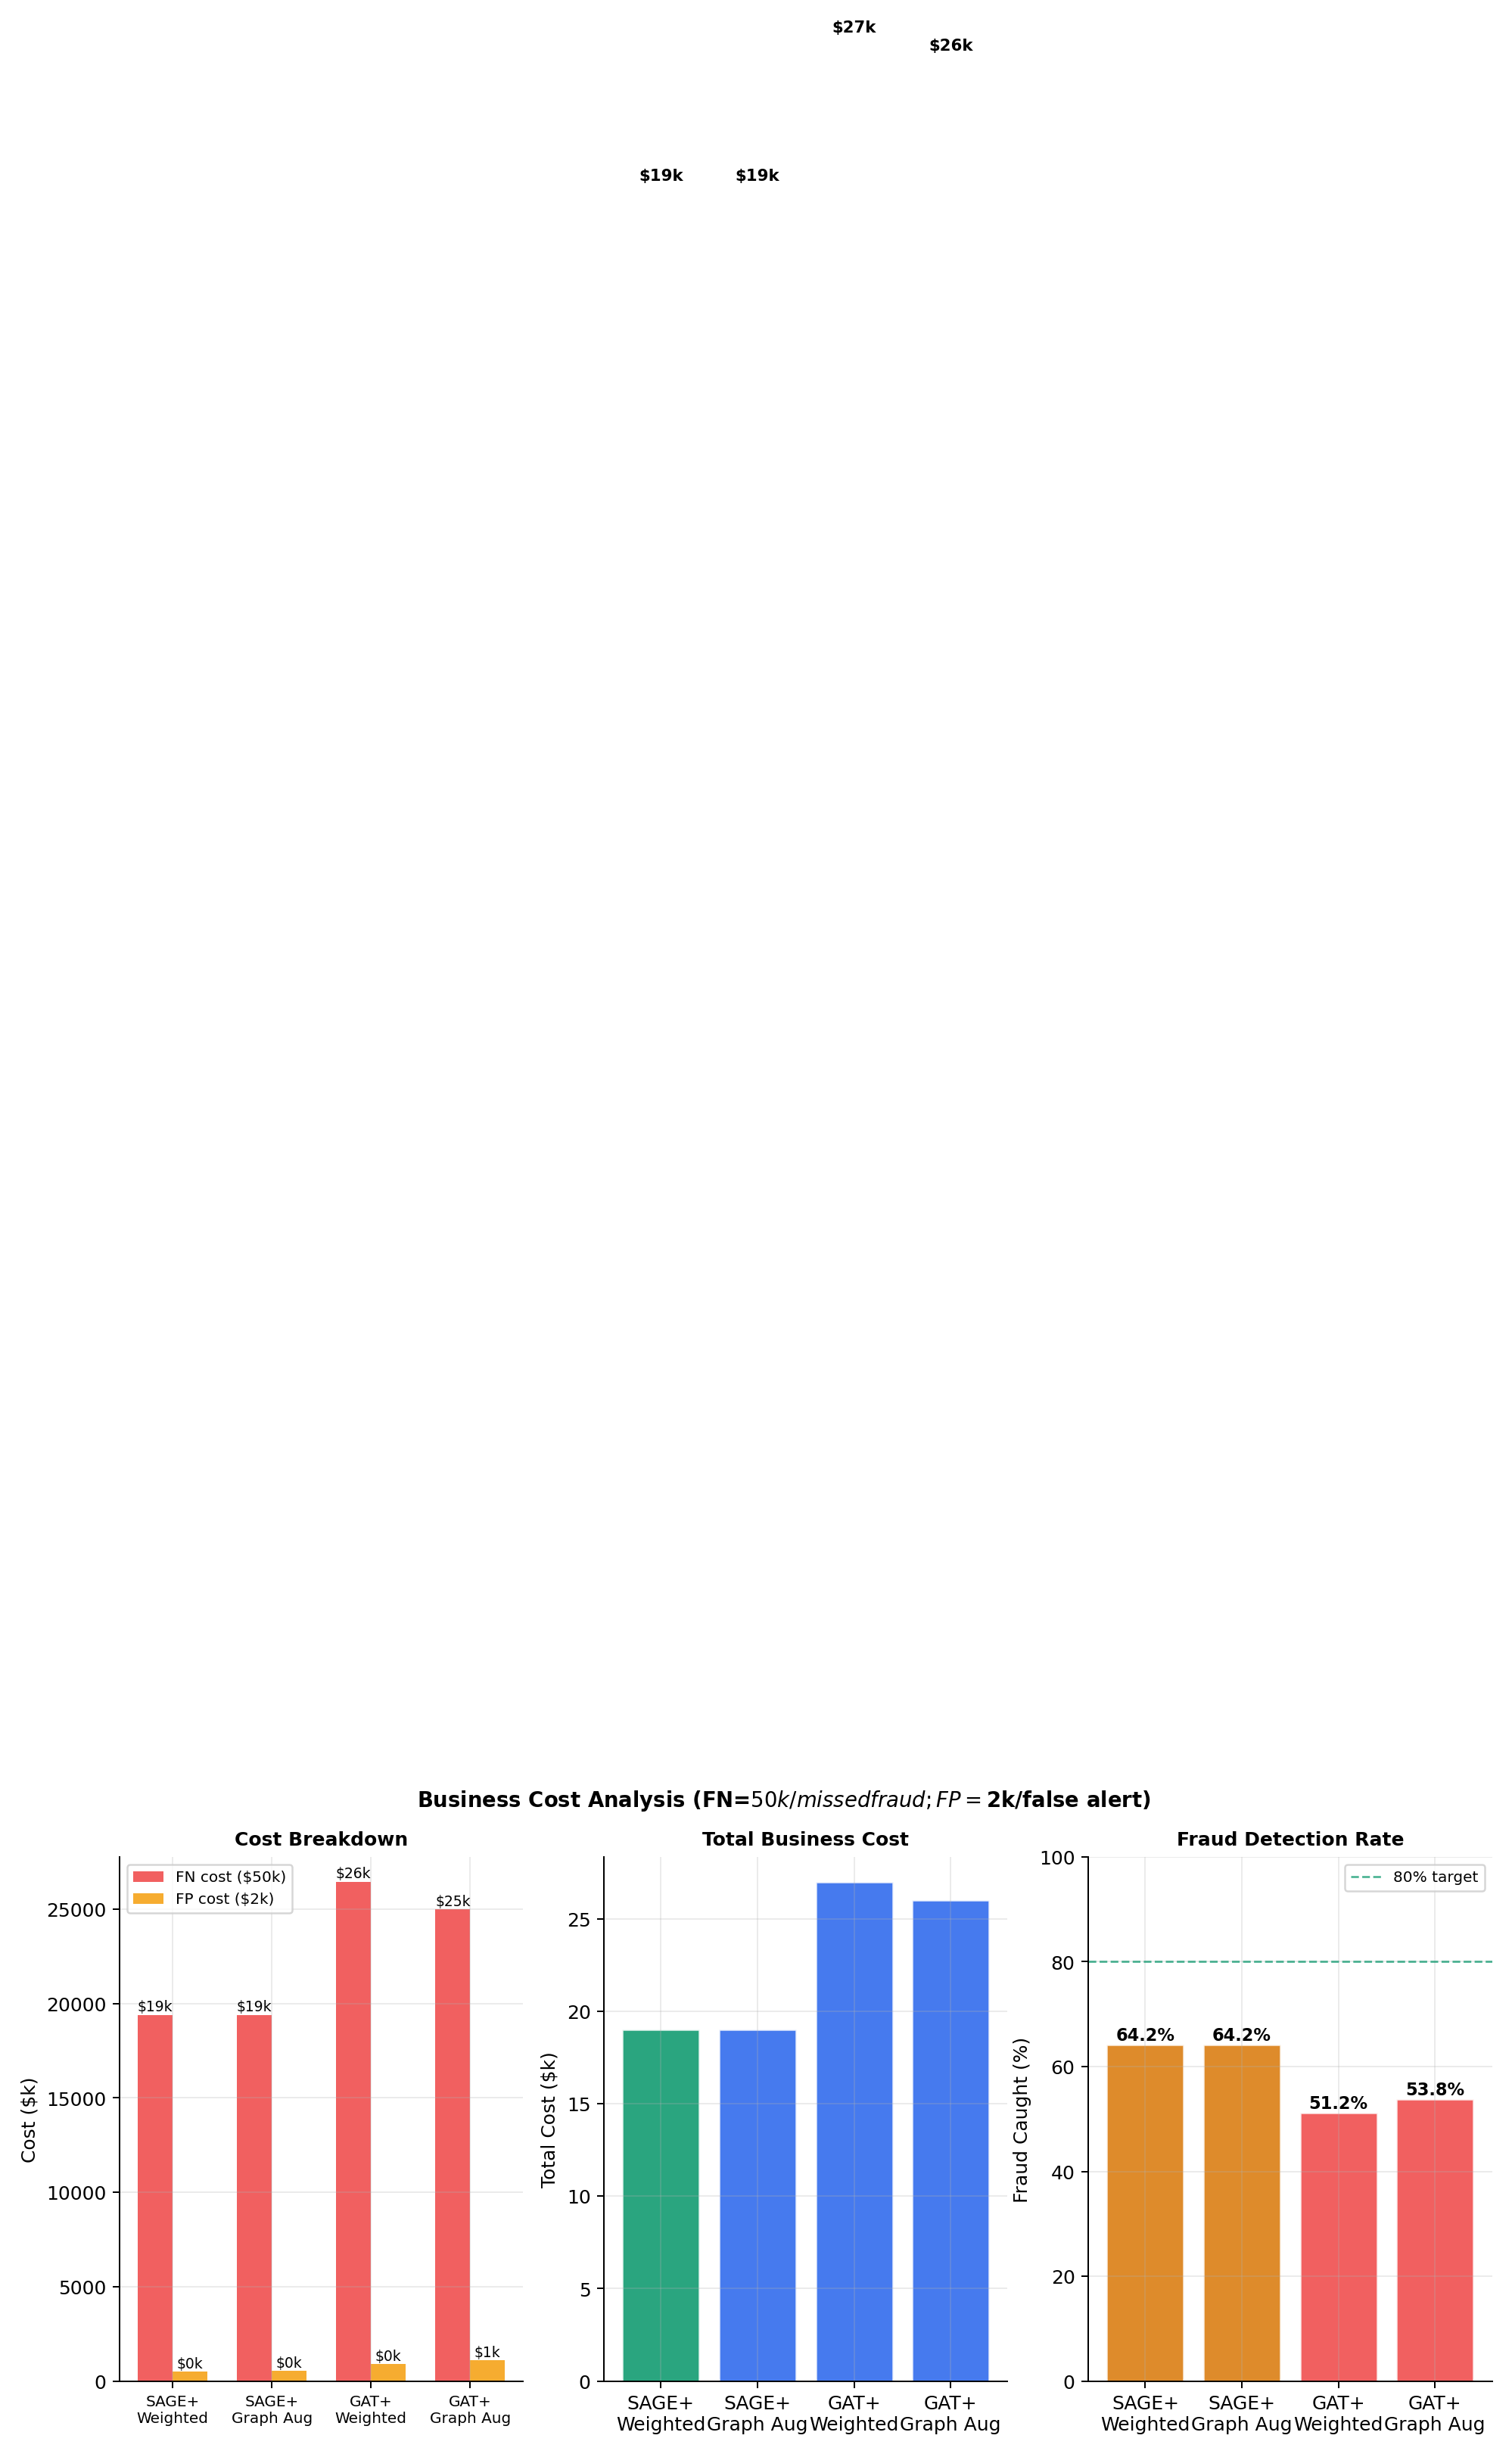
\includegraphics[width=0.82\linewidth]{fig7_business_cost.png}
\caption{Business-cost analysis under asymmetric false-negative and
false-positive penalties.}
\label{fig:business_cost}
\end{figure}

\section{Discussion and conclusion}

Three practical conclusions follow from the benchmark. First, periodic
retraining is necessary when the fraud rate moves this quickly. A static model
trained under one base rate cannot be expected to stay calibrated under another.
Second, graph structure is a conditional asset rather than a universal one. It
can help in stable periods and become harmful once the topology drifts. Third,
fraud-detection models should be selected against operational cost functions,
not against F1 alone.

The study has clear limitations. It is based on one dataset, and the inductive
pipeline uses RandomNodeLoader rather than the full neighbour-sampling setup
that would be preferable on hardware with broader support. Even with those
limitations, the main result is hard to ignore: under stricter evaluation, the
feature-only baseline is stronger and more robust than the graph models tested
here.

\FloatBarrier

\bibliographystyle{splncs04}
\bibliography{references}

\end{document}
